\section{Introducci\'on}

La navegaci\'on puede definirse como el conjunto de t\'ecnicas utilizadas para desplazarse entre un par de puntos conocidos, llamados origen y destino, siguiendo una \gls{trayectoria} tambi\'en conocida. Para esto es necesario el procesamiento de informaci\'on para conocer la posici\'on en cada momento. Ello implica poseer de alguna manera la informaci\'on necesaria y aplicarle los procedimiento y algoritmos adecuados para obtener dicha posici\'on. La manera como se obtenga la informaci\'on requerida determinar\'a el tipo de navegaci\'on que est\'a siendo utilizada.

En base a lo anterior se podr\'ia intentar una definici\'on para su aplicaci\'on aeron\'autica:

\vspace{3mm}

\begin{center}
  \begin{tikzpicture}
    \node [mybox] (box){%
      \begin{minipage}{0.90\textwidth}
	Es el conjunto de t\'ecnicas y procedimientos que permiten
        conducir eficientemente una aeronave a su lugar de destino,
        asegurando la integridad de los tripulantes, pasajeros y de
        los que est\'an en tierra. Se basa en la observaci\'on del
        cielo y del terreno y en los datos aportados por los
        instrumentos de vuelo.
      \end{minipage}
    }; \node[fancytitle, right=10pt] at (box.north west) {\bf Navegaci\'on
      A\'erea}; 
%\node[fancytitle, rounded corners] at (box.east){$\clubsuit$};
  \end{tikzpicture}%
\end{center}

\vspace{3mm}

% \colorbox{yellow!40}
% {\parbox{0.99\textwidth}
% {\bf 
% La navegaci\'on a\'erea es el conjunto de t\'ecnicas y procedimientos que permiten conducir eficientemente una aeronave a su lugar de destino, asegurando la integridad de los tripulantes y pasajeros y de los que est\'an en tierra. Se basa en la observaci\'on del cielo y el terreno y en los datos aportados por los instrumentos de vuelo.}
% }

Si bien durante mucho tiempo el t\'ermino navegaci\'on estuvo asociado esencialmente a barcos, el desarrollo de la aviaci\'on le agreg\'o una nueva dimensi\'on: adem\'as de la posici\'on horizontal (\gls{latitud} y \gls{longitud}), se necesita tambi\'en la altura de la aeronave para garantizar que no se acerca peligrosamente a alg\'un obst\'aculo. Se habla entonces de navegaci\'on 3D (\ac{3D}).

Finalmente, el gran congestionamiento del espacio a\'ereo en muchas partes del mundo hace necesario agregar otra variable m\'as: el tiempo. El tener disponible un sistema de navegaci\'on que permita mantener sincronizadas las operaciones de las aeronaves facilita el introducir m\'as aeronaves en el mismo espacio a\'ereo sin comprometer la seguridad. \'Esta es la navegaci\'on 4D, y est\'a siendo desarrollada actualmente. 

La navegaci\'on a\'erea se divide en dos tipos, dependiendo de si la aeronave es independiente o necesita de instalaciones exteriores a la aeronave para poder guiarse:

% \begin{multicols}{2}
%   \begin{itemize}
%   \item Navegaci\'on a\'erea aut\'onoma.
%   \item Navegaci\'on a\'erea no aut\'onoma.
%   \end{itemize}
% \end{multicols}


% La \textbf{navegaci\'on a\'erea aut\'onoma} es aquella que no necesita de alguna infraestructura o informaci\'on suministrada por un equipo exterior a la aeronave para poder completar con \'exito el vuelo. A su vez, \'esta se divide en:

% \begin{description}
%     \item [Navegaci\'on observada:] se basa en la observaci\'on directa por parte del navegante o piloto de las referencias necesarias en el terreno para conocer la posici\'on de la aeronave.
%     \item [Navegaci\'on a estima (Dead reckoning):] el navegante o piloto estima la posici\'on actual, conocidas la direcci\'on y la velocidad respecto al terreno.
%     \item [Navegaci\'on por fijaci\'on de la posici\'on:] \'esta a su vez se subdivide en navegaci\'on a\'erea astron\'omica, navegaci\'on a\'erea Doppler, navegaci\'on a\'erea inercial (INS = Inertial Navigation System).
% \end{description}

\begin{center}
  \begin{tikzpicture}
    \node [grupos] (box){%
      \begin{minipage}{0.90\textwidth}

	Es aquella que no necesita de alguna infraestructura o informaci\'on suministrada 
	por un equipo exterior a la aeronave para poder completar con \'exito el vuelo. 
	A su vez, \'esta se divide en:

\begin{description}
    \item [Navegaci\'on observada:] se basa en la observaci\'on directa por parte del navegante o piloto de las referencias necesarias en el terreno para conocer la posici\'on de la aeronave.
    \item [Navegaci\'on a estima (Dead reckoning):] el navegante o piloto estima la posici\'on actual, conocidas la direcci\'on y la velocidad respecto al terreno.
    \item [Navegaci\'on por fijaci\'on de la posici\'on:] \'esta a su vez se subdivide en navegaci\'on a\'erea astron\'omica, navegaci\'on a\'erea Doppler, navegaci\'on a\'erea inercial (INS = Inertial Navigation System).
\end{description}

    \end{minipage}
  }; \node[fancytitle.grupos] at (box.north) {\bf Navegaci\'on A\'erea Aut\'onoma};
\end{tikzpicture}
\end{center}

\begin{center}
  \begin{tikzpicture}
    \node [grupos] (box){%
      \begin{minipage}{0.90\textwidth}

 necesita de instalaciones exteriores para su guiado durante el vuelo, estas reciben el nombre de \emph{ayudas a la navegaci\'on}. Estas ayudas se pueden dividir a su vez dependiendo del tipo de informaci\'on que transmiten as\'i como del canal a trav\'es del cual lo hacen. As\'i, las ayudas pueden ser:

\begin{description}
    \item [Ayudas visuales al aterrizaje:] son instalaciones que proporcionan se\~nales visuales durante la etapa de aterrizaje de la aeronave.
    \item [Radioayudas:] Se basan en se\~nales radioel\'ectricas, usualmente generadas en instalaciones terrestres y recibidas a bordo.
    \item [Navegaci\'on por sat\'elite:] se basa en una constelaci\'on de sat\'elites que transmite rangos de se\~nales utilizados para el posicionamiento y localizaci\'on en cualquier parte del globo terrestre, ya sea en tierra, mar o aire. Estos permiten determinar las coordenadas geogr\'aficas y la altitud de un punto dado como resultado de la recepci\'on de se\~nales provenientes de dicha constelaci\'on.
\end{description}

    \end{minipage}
  }; 
\node[fancytitle.grupos] at (box.north) {\bf Navegaci\'on A\'erea No Aut\'onoma};
\end{tikzpicture}
\end{center}


\begin{figure}[!h]
  \centering
  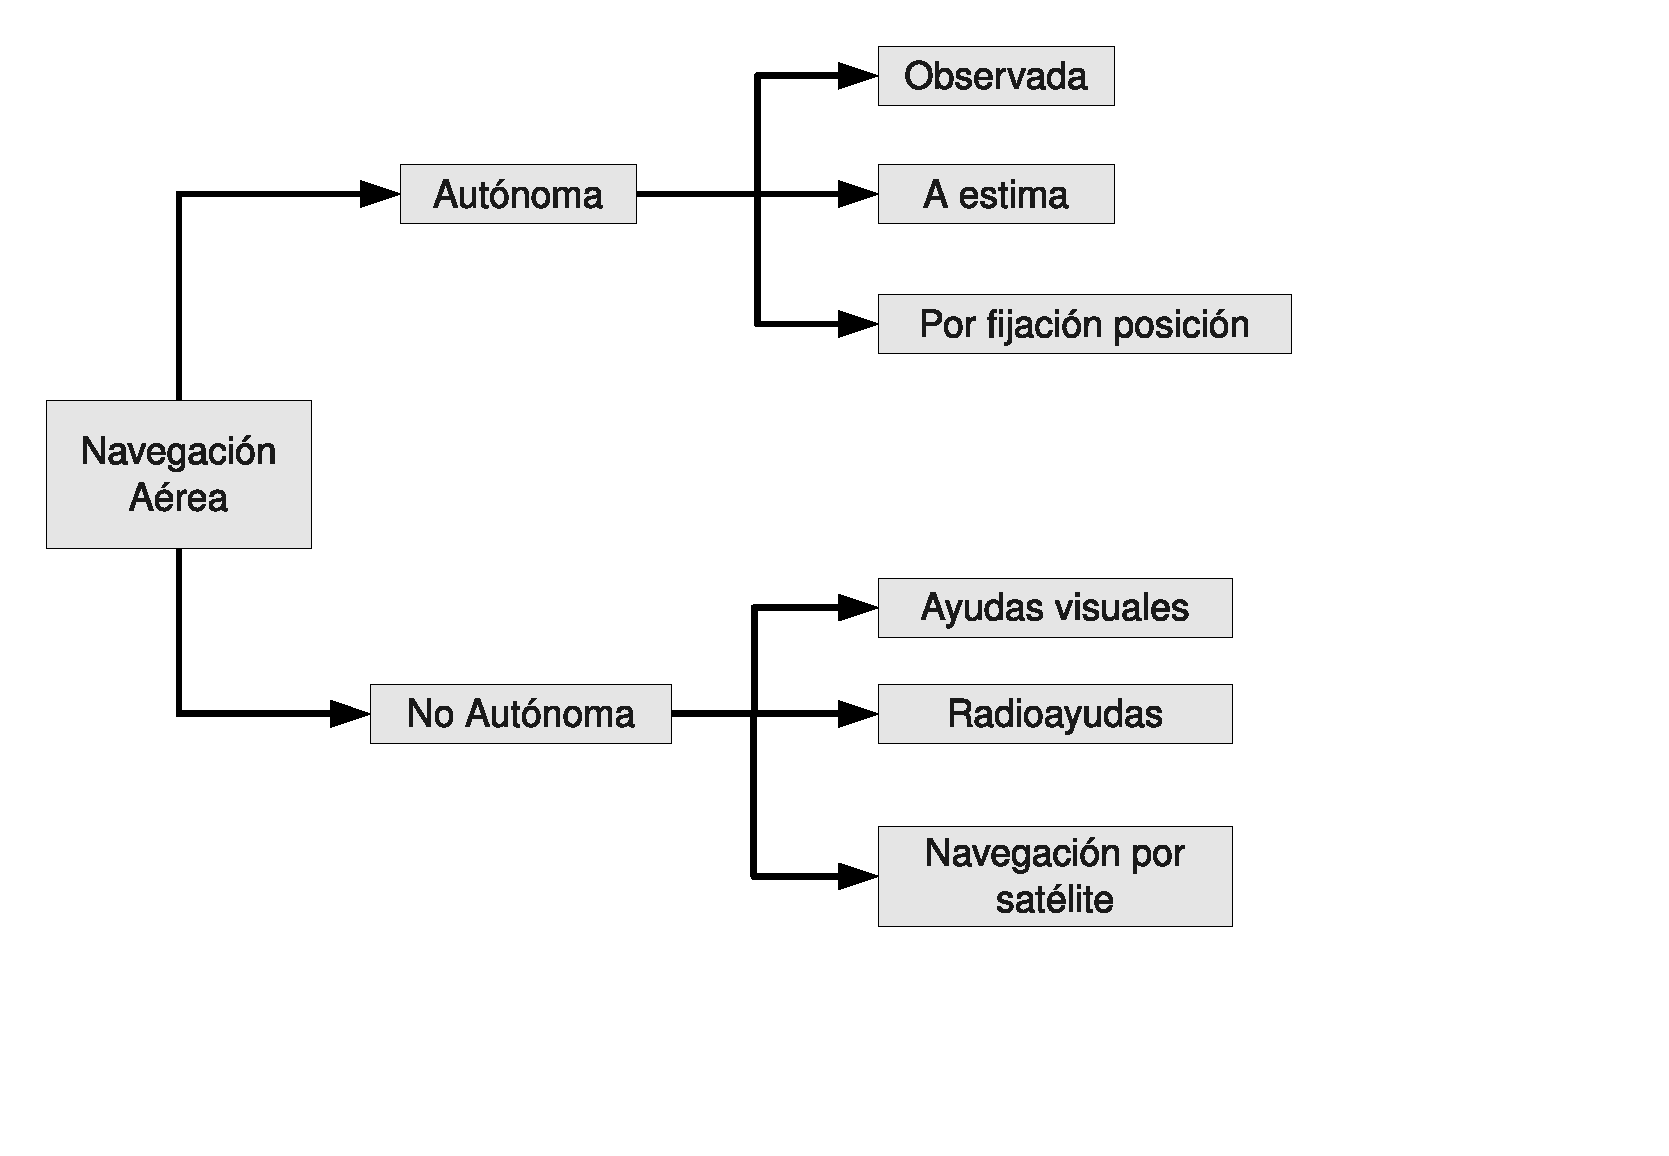
\includegraphics[width=\textwidth]{Imagenes/06.00.navegacion/tipos-navegacion.eps}
  \caption{Navegaci\'on A\'erea}
  \label{fig:navegacion.aerea.cuadro}
\end{figure}




\section{M\'etodos de Navegaci\'on A\'erea}

\subsection{Navegaci\'on Aut\'onoma}

\subsubsection{Navegaci\'on Observada \cite{Aena_SENASA_nav_aerea} }

 Es la que se realiza bas\'andose en
referencias del terreno que hay que ver, es una navegaci\'on visual.
Se trata de que el piloto localice las referencias del terreno, para lo
cual es fundamental el uso de buenos 
\begin{minipage}[b]{0.650\linewidth}
mapas en los que vengan
reflejados con claridad los accidentes geogr\'aficos, los pueblos y
ciudades, las carreteras y las v\'ias del ferrocarril, etc. \cite{Aena_SENASA_nav_aerea}

  Para este tipo de navegaci\'on se debe preparar el vuelo,
  estableciendo con toda precisi\'on la ruta que se va a seguir sobre
  el propio mapa.

  En el mismo mapa se marcan puntos en la ruta para dividirla por
  tramos, tratando de que las marcas coincidan con puntos de
  referencia de la ruta. Se deben calcular los tramos por kil\'ometros
  y tiempo que se tarda en volar de un punto a otro.

  Hay que tener buena informaci\'on meteorol\'ogica de toda la ruta y
  llevar la lista de las frecuencias de Torres y Centros de control.
  Si se encontrase perdido, basarse en la \'ultima posici\'on que se
  reconoci\'o y calcular la posici\'on probable por el tiempo
  transcurrido; en esa posici\'on probable tratar de reconocer alguna
  referencia significativa.

\end{minipage}
\begin{minipage}[b]{0.350\linewidth}
\centering
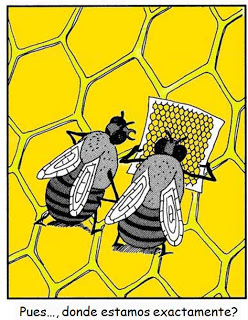
\includegraphics[width=0.9\textwidth]{Imagenes/06.00.navegacion/donde_estamos.jpg}  
\end{minipage}


%Establecer contacto por radio con la Torre o Centro de control m\'as apropiado y tratar de obtener marcaciones de radiogonometr\'ia pulsando el bot\'on del micr\'ofono de la radio, lo cual permitir\'ia al controlador dar una marcaci\'on QDM (rumbo a la estaci\'on), para llegar a alg\'un aeropuerto.



\subsubsection{Navegaci\'on a Estima (Dead Reckoning) \cite{Salazar_nav_aerea}}

  Dead reckoning es traducido en espa\~nol como ``\textit{navegacion
    por estima}'', es una expresi\'on derivada del t\'ermino n\'autico
  \textit{deduced reckoning} (c\'alculo basado en inferencia), y es un
  procedimiento matem\'atico que utiliza sencillas f\'ormulas
  trigonom\'etricas para inferir la ubicaci\'on actual de un nav\'io
  haciendo c\'alculos basados en el rumbo y la velocidad de
  navegaci\'on a lo largo de un per\'iodo de tiempo, sin usar el cielo
  y los astros como referencia.

  \begin{minipage}[b]{0.650\linewidth}
  

  La amplia mayor\'ia de sistemas de robots m\'oviles terrestres que
  se usan hoy en d\'ia, utilizan la t\'ecnica dead reckoning como
  columna vertebral de su estrategia de navegaci\'on, y al igual que
  sus hom\'ologos n\'auticos, necesitan eliminar los errores
  acumulados con continuos ajustes con varios sistemas de ayuda a la
  navegaci\'on.


  El principal problema que tiene la navegaci\'on a estima es que
  requiere la selecci\'on de una serie de puntos significativos de la
  ruta que tienen que estar
 a la vista de la tripulaci\'on, aunque en
  ocasiones estas referencias visuales no se obtienen, especialmente
  en vuelos nocturnos o con condiciones atmosf\'ericas adversas y en
  vuelos realizados sobre el mar.

\end{minipage}
\begin{minipage}[b]{0.35\linewidth}
    \centering
    
     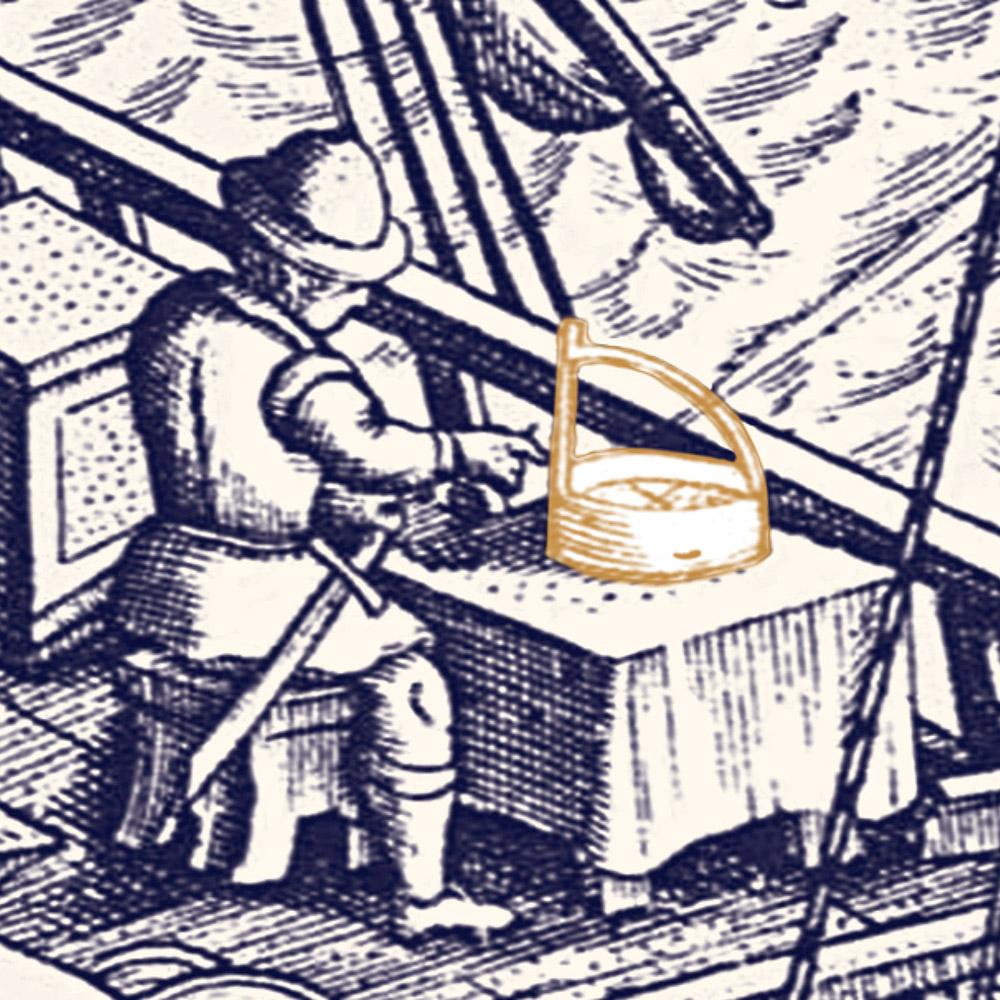
\includegraphics[width=0.90\textwidth]{Imagenes/06.00.navegacion/marinero-navegacion.jpg}
   \end{minipage}
%   \begin{minipage}[b]{0.50\linewidth}
% 	\centering
%   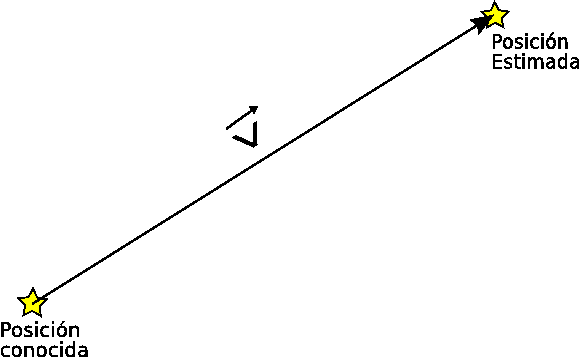
\includegraphics[keepaspectratio,width=0.9\textwidth]{./Imagenes/06.00.navegacion/dead-reckoning.png}
  
%   \end{minipage}
% %     \caption{Dead recokning en la navegaci\'on mar\'itima}
% % \label{fig:dead.reckoning.navegacion.maritima}
% % \end{figure}


  La implementaci\'on m\'as simple posible de la t\'ecnica dead
  reckoning es habitualmente llamada \emph{odometr\'ia}, t\'ermino que
  implica que el desplazamiento de un veh\'iculo a lo largo de la
  \gls{trayectoria} se deriva directamente de alg\'un od\'ometro o
  cuentarrevoluciones a bordo del veh\'iculo. Una t\'ecnica com\'un
  para implementar la odometr\'ia consiste en utilizar encoders
  \'opticos directamente acoplados a los motores o a los ejes de las
  ruedas.


\begin{figure}[!h]
  \centering
  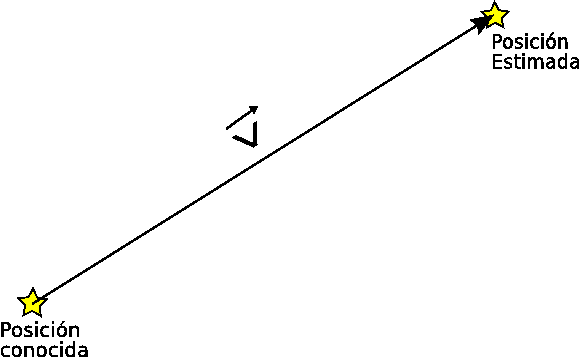
\includegraphics[keepaspectratio,width=0.7\textwidth]{./Imagenes/06.00.navegacion/dead-reckoning.png}
  \caption{Navegaci\'on a estima \cite{Salazar_nav_aerea}}
  \label{fig:dead-reckoning}
\end{figure}


Si, dado un marco de referencia arbitrario, las coordenadas de la posici\'on previa conocida $P_1$ son $(x_1, y_1)$ y las de la nueva posici\'on $P_2$ son $(x_2, y_2)$, entonces el vector que une ambas posiciones se puede denotar como $\vec x_{12}$, y en notaci\'on vectorial:


  \begin{equation}
\vec x_{12} = \vec x_2 - \vec x_1 = (x_2, y_2) - (x_1, y_1) = (x_2 - x_1, y_2 - y_1)
    \label{eq:dead-reckoning-vtor-posicion}
  \end{equation}



En forma matricial se expresar\'ia como:


\begin{equation}\label{eq:dead-reckoning-expresion-matricial}
 \vec x_{12} = \vec x_2 - \vec x_1 = 
\left\{ \begin{array}{c} x_2 \\ y_2 \end{array} \right\} 
- \left\{ \begin{array}{c} x_1 \\ y_1 \end{array} \right\} 
=
\left\{ \begin{array}{c} x_2 - x_1 \\ y_2 - y_1 \end{array} \right\}
\end{equation}

Y entonces, la navegaci\'on a estima implica que:

\begin{equation}
  \label{eq:dead-reckoning-otra-expresion}
\vec x_2 = \vec x_1 + \vec x_{12} = \vec x_1 + \int_{t_1}^{t_2} \vec v_{12} dt = \vec x_1 + \int_{t_1}^{t_2} \vec v dt   
\end{equation}

N\'otese que en la expresi\'on (\ref{eq:dead-reckoning-otra-expresion}) se asume que el vector $\vec x_{12}$ es igual a la integraci\'on del vector velocidad estimada $\vec v$. Esto no necesariamente es as\'i, debido a que el vector velocidad estimada $\vec v$ no necesariamente es igual al vector velocidad real $\vec v_{12}$. Esto en general se debe a:

\begin{minipage}[b]{0.70\linewidth}
  \begin{itemize}
  \item Una componente adicional a la velocidad del avi\'on, causada
    t\'ipicamente, por el viento ($v_w$). La acci\'on del viento, si
    no est\'a alineada con la velocidad del avi\'on, lo saca de su
    curso deseado (track).

  \item Por otra parte, si el viento est\'a alineado, pero en contra,
    causar\'a una sobre-estimaci\'on (overshoot) de la posici\'on (se
    estimar\'a que la aeronave est\'a m\'as all\'a de donde realmente
    est\'a), y si est\'a a favor causar\'a una sub-estimaci\'on
    (undershoot) de la posici\'on.

  \item Un error del sistema de navegaci\'on. Los errores m\'as
    perniciosos en este sentido son los \textbf{errores
      sistem\'aticos}, que son aquellos en los que hay un sesgo (o
    bias) que continuamente altera la medida en una misma direcci\'on
    (causando, por ejemplo, una desviaci\'on constante hacia la
    derecha de 0.1º por minuto).

  \end{itemize}
\end{minipage}
\begin{minipage}[b]{0.30\linewidth} \centering
  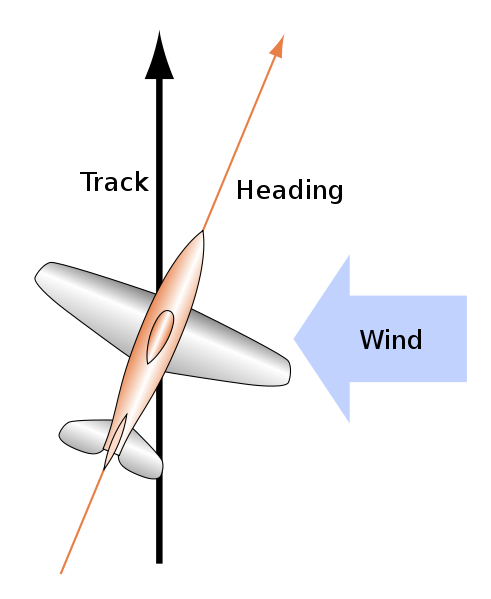
\includegraphics[width=0.85\textwidth]{Imagenes/06.00.navegacion/ajuste-viento.png}
	\captionof{figure}{El efecto del viento}
\end{minipage}

\begin{figure}[!h]
  \centering
  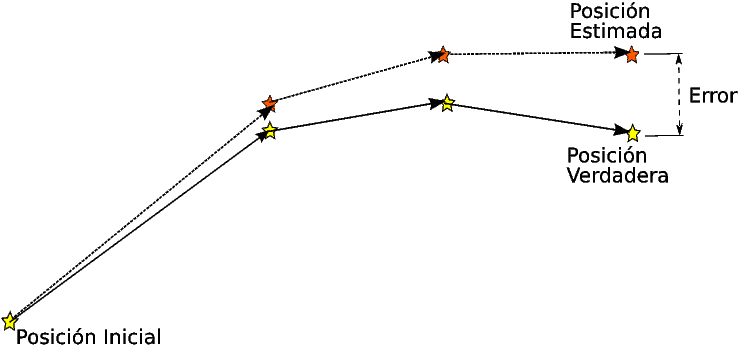
\includegraphics[keepaspectratio,width=0.8\textwidth]{./Imagenes/06.00.navegacion/dead-reckoning-error.png}  
  \caption{Error acumulativo en la navegaci\'on a estima \cite{Salazar_nav_aerea}}
  \label{fig:dead-reckoning-error}
\end{figure}

      
Debido al proceso de integraci\'on impl\'icito en este tipo de navegaci\'on, se tiene el inconveniente de que \textbf{los errores son acumulativos}, es decir, una peque\~na desviaci\'on en las estimaciones iniciales de la posici\'on se va convirtiendo con el paso del tiempo en un gran error, tal y como indica la Figura \ref{fig:dead-reckoning-error}.


Es por esta raz\'on que la navegaci\'on a estima debe combinarse con otros tipos de navegaci\'on (el visual, por ejemplo) para obtener una correcci\'on de la posici\'on que permita empezar una iteraci\'on ``\textit{fresca}'' del m\'etodo (es decir, cada cierto tiempo hace falta obtener un correcci\'on confiable).

Tambi\'en es conveniente acotar que la navegaci\'on a estima en aeron\'autica se usa para conocer la posici\'on en 2D.


\subsubsection{Navegaci\'on por Fijaci\'on de la Posici\'on}

%Se habla de navegaci\'on aut\'onoma cuando \'esta se realiza sin necesidad de utilizar se\~nales emitidas por transmisores de referencia en la tierra o en el espacio. Al principio se requiere partir de una posici\'on conocida y en la pr\'actica es necesario cotejar los resultados cada cierto tiempo usando otro tipo de navegaci\'on.


\begin{description}


\item[Navegaci\'on A\'erea Astron\'omica:] hace uso de la astronom\'ia para el uso directo del navegante a\'ereo, que comprende principalmente las coordenadas celestes, el tiempo y la posici\'on y movimiento aparente de los astros con respecto a la Tierra.

  \begin{minipage}[b]{0.60\linewidth}
    Se emplea en vuelos de larga distancia donde se carece de radio
    ayudas convenientes. Para utilizarla se requiere disponer de
    sextante, cron\'ometro, almanaque a\'ereo y tabla de
    reducci\'on. La combinaci\'on de los diferentes m\'etodos de
    navegaci\'on permite resolver el problema de navegaci\'on con
    mayor facilidad.

Con la evoluci\'on y desarrollo de las aeronaves, as\'i como el aumento de la autonom\'ia de vuelo, se hizo patente la necesidad de nuevos sistemas de posicionamiento que permitieran atravesar  zonas en las cuales las radio ayudas
  \end{minipage}
  \begin{minipage}[b]{0.40\linewidth} \centering
    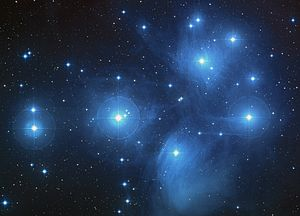
\includegraphics[width=0.85\textwidth]{Imagenes/06.00.navegacion/pleyades}
	\captionof{figure}{Las Pl\'eyades}
  \end{minipage}
 existentes no llegaban (por ejemplo en el mar). Para superar este problema se ech\'o mano de la navegaci\'on mar\'itima, la cual dispon\'ia desde muy antiguo de una t\'ecnica para establecer la posici\'on de un punto a partir de la observaci\'on de los astros. Para ello se utilizaban instrumentos tales como el astrolabio y el sextante. El Astrolabio permite localizar las posiciones de las estrellas sobre la b\'oveda celeste y se utilizaba para determinar la altura, la posici\'on y el movimiento de los astros sobre el horizonte. Este instrumento, tan antiguo y complejo, tiene adem\'as otro tipo de aplicaciones, como son: determinar la hora del d\'ia o de la noche, mediante la observaci\'on del Sol o de un Astro sobre el horizonte; calcular la hora de salida de las estrellas; as\'i como resolver problemas astrol\'ogicos m\'as complejos. 

 % \begin{figure}[!h]
 %   \centering
 %   \subfigure[Astrolabio]{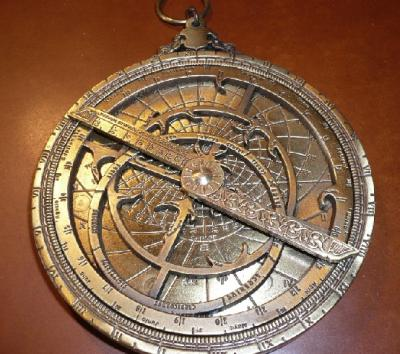
\includegraphics[height=6cm]{Imagenes/06.00.navegacion/astrolabio.jpg}}
 %   \subfigure[Sextante]{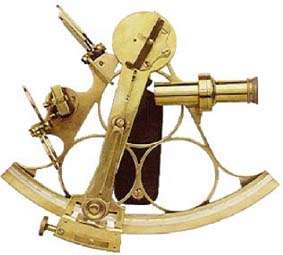
\includegraphics[height=6cm]{Imagenes/06.00.navegacion/sextante.jpg}   
 %   \caption{Instrumentos para navegaci\'on mar\'itima}
 %   \label{fig:instrumentos.navegacion.maritima}
 % \end{figure}

Poco tiempo despu\'es se invent\'o el sextante, que se basa en los mismos principios que el astrolabio pero se vale de dos nuevos elementos: un largavistas y un juego de espejos, cuyo uso de precisi\'on resultaron efectivos despu\'es de los estudios sobre \'optica. El sextante es un instrumento que permite medir \'angulos entre dos objetos tales como dos puntos de una costa o un astro -tradicionalmente el Sol- y el horizonte. Conociendo la elevaci\'on del Sol y la hora del d\'ia se puede determinar la latitud a la que se encuentra el observador. Esta determinaci\'on se efect\'ua con bastante precisi\'on mediante c\'alculos matem\'aticos sencillos de aplicar.

La navegaci\'on astron\'omica jug\'o un papel de complemento para la navegaci\'on a estima y sirvi\'o b\'asicamente para determinar la posici\'on cuando no era posible establecer referencias visuales con el terreno. Esta t\'ecnica de realizar peri\'odicamente la fijaci\'on de la posici\'on permiti\'o las m\'as importantes proezas registradas en el progreso de la aviaci\'on.

Por otra parte, los c\'alculos a realizar, a\'un con la utilizaci\'on de unos m\'etodos muy elaborados, exig\'ian una dedicaci\'on que no era compatible con la atenci\'on que la tripulaci\'on hab\'ia de destinar al control de la aeronave en vuelo. Esta situaci\'on supuso la aparici\'on del navegante como miembro adicional de la tripulaci\'on, capaz de establecer varias veces la posici\'on del avi\'on bas\'andose en la observaci\'on con sextante, de determinados cuerpos celestes y el empleo de almanaques que indicaban su posici\'on en las diferentes \'epocas del a\~no.




\item[Navegaci\'on A\'erea Doppler:] es un sistema de radar, el cual suministra a la tripulaci\'on, con alto grado de precisi\'on, la velocidad y el \'angulo de desviaci\'on (deriva) durante el vuelo a la vez que suministra datos visuales (lecturas) en millas n\'auticas, que lo separan del destino y millas que lo alejan a la izquierda o a la derecha del curso preseleccionado.

El sistema opera continua y autom\'aticamente sin la ayuda de estaciones de tierra. Fue dise\~nado utilizando el \textbf{Efecto Doppler}\footnote{ El \textbf{Efecto Doppler} es llamado as\'i por el austr\'iaco Christian Doppler consiste en la variaci\'on de la longitud de onda de cualquier tipo de onda emitida o recibida por un objeto en movimiento. Doppler propuso este efecto en 1842 en una monograf\'ia titulada Über das farbige Licht der Doppelsterne und einige andere Gestirne des Himmels (``Sobre el color de la luz en estrellas binarias y otros astros''). } ; recordando el mismo principio f\'isico de comportamiento de un objeto que se aproxima y se aleja: ``Que la frecuencia de una se\~nal observada a un punto fijo en el espacio es mayor que la observada en una fuente de se\~nal, si la fuente est\'a en movimiento hacia el punto fijo.''     Rec\'iprocamente, la frecuencia en el punto fijo ser\'a menor entonces que en la fuente, si la fuente se est\'a moviendo lejos del punto fijo.

Este aumento o disminuci\'on en frecuencia es proporcional a la velocidad a la cual la fuente de se\~nal se est\'a moviendo y si \'esta es constantemente monitoreada y medida por algunos m\'edios de precisi\'on, la informaci\'on obtenida puede ser usada para determinar el curso y la velocidad de la misma fuente de se\~nal.

En este caso, la fuente de se\~nal en el avi\'on es el mismo sistema DOPPLER y es este sistema igualmente el que constantemente monitorea y mide la se\~nal, la cual es reflejada en la superficie terrestre.

Usualmente se instalan dos sistemas en un avi\'on y consiste de una antena (usada para ambos sistemas), un TRANSCEPTOR (transmisor - receptor), una unidad seguidora (Tracker), un panel de control, un computador (no como lo conocemos actualmente), un controlador del computador y un indicador.

Cada sistema recibe informaci\'on de rumbo de uno de los dos sistemas de comp\'as y suministra al sistema de piloto autom\'atico informaci\'on de cualquiera de los sistemas DOPPLER.

Ambos sistemas operan simult\'aneamente y separadamente aunque reciben se\~nales de informaci\'on de una antena com\'un.



\item[Navegaci\'on A\'erea Inercial \cite{Salazar_nav_aerea}:] consiste en una plataforma estabilizada con gir\'oscopos que sirve como marco de referencia. En la misma unos aceler\'ometros y gir\'oscopos permiten medir los cambios de velocidad (tanto traslacional como rotacional) y, mediante integraci\'on sucesiva de los datos, obtener la posici\'on de la aeronave y su \gls{actitud}.
% , como se indica en las siguientes expresiones:


% \[
%  \begin{array}{l} \vec v(t) - \vec v_0 = \displaystyle \int_{t_0}^{t} \vec ... ...\\ \vec x(t) - \vec x_0 = \displaystyle \int_{t_0}^{t} \vec v dt \end{array}
% \]


% \[
%  \begin{array}{l} \vec \omega(t) - \vec \omega_0 = \displaystyle \int_{t_0}... ...(t) - \vec \theta_0 = \displaystyle \int_{t_0}^{t} \vec \omega dt \end{array}
% \]

% Donde:

%     * $\vec a$: Vector aceleraci\'on traslacional.

%     * $\vec v$: Vector velocidad traslacional.

%     * $\vec v$: Vector posici\'on.

%     * $\vec \alpha$: Vector aceleraci\'on angular.

%     * $\vec \omega$: Vector velocidad angular.

%     * $\vec \theta$: Vector posici\'on angular.

%Notese que, seg\'un las expresiones anteriores, 

En realidad se est\'a llevando a cabo un sofisticado proceso de dead reckoning  y que, debido a que la plataforma giro-estabilizada no es perfecta, en los c\'alculos se van introduciendo errores acumulativos que deben ser corregidos mediante fuentes externas al cabo de un cierto tiempo de vuelo.

Dicho tiempo es variable seg\'un la calidad del INS utilizado, un sistema de buena calidad acumula un error en distancia de un kil\'ometro o menos por hora, y el error angular t\'ipicamente es menor a pocas d\'ecimas de grado por hora. 

\end{description}

\subsection{Navegaci\'on A\'erea No Aut\'onoma}

\subsubsection{Ayudas visuales}

Utilizadas casi desde los inicios mismos de la aviaci\'on, por lo general est\'an asociadas a la operaci\'on de aterrizaje:
\begin{description}
\item [De punto fijo] Permiten identificar f\'acilmente desde lo lejos un punto de referencia importante. El faro aeron\'autico es el ejemplo t\'ipico.

    \item [De direcci\'on] Proporcionan al piloto informaci\'on valiosa sobre la direcci\'on de, por ejemplo, el viento (manga de viento) o el eje de la pista (luces de eje de pista).

    \item [De elevaci\'on] En este caso se indica al piloto el \'angulo vertical con el que se aproxima a la pista. Entran en esta categor\'ia los sistemas de luces PAPI (ver Figura \ref{fig:papi}), VASI, etc.

\end{description}
     

En la Figura \ref{fig:papi} se muestra el t\'ipico emplazamiento de un sistema PAPI. 



\subsubsection{Radioayudas}

Las radioayudas se pueden clasificar seg\'un el tipo de informaci\'on que proporcionan:

\begin{description}
\item [Direcci\'on a un punto fijo] Este tipo de ayudas simplemente indica, mediante una aguja, la direcci\'on en la que tendr\'ia que volar el piloto para llegar a un punto de referencia dado. A este tipo pertenece el sistema ADF/NDB.

    \item [Azimutales] El azimut es el \'angulo horizontal formado entre un eje de referencia (por ejemplo el vector radioayuda norte magn\'etico), y el vector radioayuda aeronave. En esta clasificaci\'on entran, entre otros, el VOR y el ILS/LLZ.
      Usar una radioayuda azimutal a menudo se de\-no\-mi\-na navegaci\'on theta ($\theta$), por la notaci\'on que recibe habitualmente el \'angulo proporcionado (azimut).

    \item [Cenitales] En este caso se proporciona el \'angulo vertical entre el eje de referencia radioayuda-horizonte y el vector radioayuda-aeronave. El ILS/GS es el ejemplo t\'ipico.

    \item [De distancia] Este tipo de ayudas proporcionan la distancia entre radioayuda y aeronave. Como esta distancia a menudo se denota como ``rho'' ($\rho$), se habla entonces de navegaci\'on rho. A esta categor\'ia pertenece el DME.

\end{description}
     
En la Figura \ref{fig:DVOR-vista-aerea} se presenta la vista a\'erea de una estaci\'on VOR en B\'elgica. 



\begin{figure}[!h]
  \centering

\subfigure[Precision Approach Path Indicator - PAPI \cite{wikipedia_esp} ]{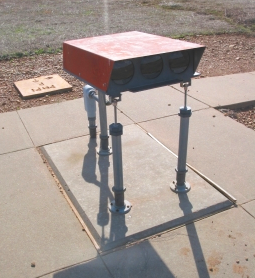
\includegraphics[keepaspectratio,height=7cm]{./Imagenes/06.00.navegacion/papi.png}
  \label{fig:papi}}
\subfigure[Vista a\'erea de un VOR \cite{wikipedia_esp}]{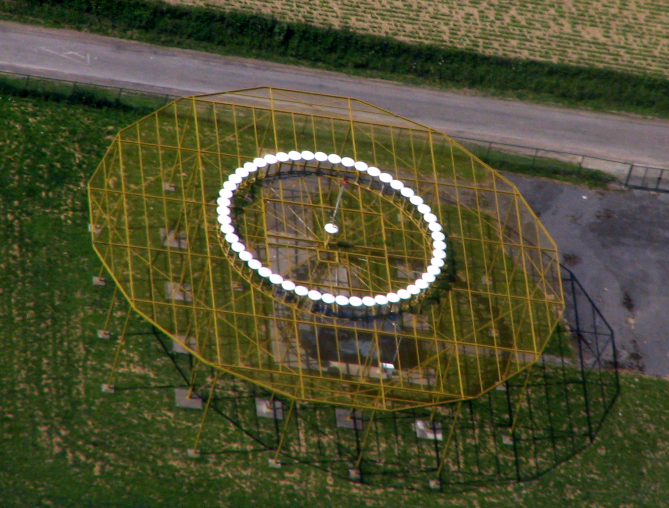
\includegraphics[keepaspectratio,height=7cm]{./Imagenes/06.00.navegacion/DVOR-aerea.png}
  \label{fig:DVOR-vista-aerea}}

\caption{Ayudas visuales}
\end{figure}




\subsubsection{Navegaci\'on por sat\'elite}

Los \'ultimos avances en la tecnolog\'ia espacial est\'an generando una revoluci\'on en la manera como se realiza la navegaci\'on. De hecho, se estima que antes del 2020 los sistemas basados en navegaci\'on por sat\'elite sustituir\'an a casi todos los dem\'as sistemas utilizados actualmente.

Estos sistemas reciben el nombre gen\'erico de GNSS (Global Navigation Satellite Systems) porque su cobertura es mundial. Los representantes m\'as importantes son:

\begin{description}
\item [GPS] Sistema estadounidense de origen militar, es actualmente el m\'as conocido y desarrollado. Empez\'o a operar a principios de la d\'ecada de 1980 y se est\'an ejecutando planes para su modernizaci\'on.% La Figura \ref{fig:satelite-GPS} es una representaci\'on art\'istica de un sat\'elite GPS de la generaci\'on IIF.
 En 1957 la Uni\'on Sovi\'etica lanz\'o al espacio el sat\'elite Sputnik I, que era monitorizado mediante la observaci\'on del Efecto Doppler de la se\~nal que transmit\'ia. Debido a este hecho, se comenz\'o a pensar que, de igual modo, la posici\'on de un observador podr\'ia ser establecida mediante el estudio de la frecuencia Doppler de una se\~nal transmitida por un sat\'elite cuya \'orbita estuviera determinada con precisi\'on.
La Armada estadounidense r\'apidamente aplic\'o esta tecnolog\'ia, para proveer a los sistemas de navegaci\'on de sus flotas de observaciones de posiciones actualizadas y precisas. As\'i surgi\'o el sistema TRANSIT, que qued\'o operativo en 1964, y hacia 1967 estuvo disponible, adem\'as, para uso comercial.
Las actualizaciones de posici\'on, en ese entonces, se encontraban disponibles cada 40 minutos y el observador deb\'ia permanecer casi est\'atico para poder obtener informaci\'on adecuada.
Posteriormente, en esa misma d\'ecada y gracias al desarrollo de los relojes at\'omicos, se dise\~n\'o una constelaci\'on de sat\'elites, portando cada uno de ellos uno de estos relojes y estando todos sincronizados con base en una referencia de tiempo determinada.
En 1973 se combinaron los programas de la Armada y el de la Fuerza A\'erea de los Estados Unidos (este \'ultimo consistente en una t\'ecnica de transmisi\'on codificada que prove\'ia datos precisos usando una se\~nal modulada con un c\'odigo de ruido pseudo-aleatorio (PRN = Pseudo-Random Noise), en lo que se conoci\'o como Navigation Technology Program, posteriormente renombrado como NAVSTAR GPS.
Entre 1978 y 1985 se desarrollaron y lanzaron once sat\'elites prototipo experimentales NAVSTAR, a los que siguieron otras generaciones de sat\'elites, hasta completar la constelaci\'on actual, a la que se declar\'o con «capacidad operacional inicial» en diciembre de 1993 y con «capacidad operacional total» en abril de 1995.
En 1994, este pa\'is ofreci\'o el servicio normalizado de determinaci\'on de la posici\'on para apoyar las necesidades de la OACI, y esta acept\'o el ofrecimiento.

    \item [GLONASS] La respuesta sovi\'etica al GPS, con las dificultades econ\'omicas de la ex-URSS cay\'o a niveles de inoperatividad. Sin embargo, hay planes de reactivarlo gracias a la ayuda de la Uni\'on Europea.

Los tres primeros satelites fueron colocados en \'orbita en octubre de 1982. El sistema fue pensado para ser funcional en el a\~no 1991, pero la constelaci\'on no fue terminada hasta diciembre de 1995 y comenz\'o a ser operativo el 18 de enero de 1996. Ese mismo a\~no la ya Federaci\'on Rusa ofreci\'o el canal de exactitud normalizada (CSA) del GLONASS para apoyar las necesidades de la OACI, y \'esta acept\'o el ofrecimiento.

La situaci\'on econ\'omica de Rusia a partir de 1990 supuso que en abril de 2002 s\'olo 8 sat\'elites estuvieran completamente operativos.

En el 2004, 11 sat\'elites se encontraban en pleno funcionamiento. A fines de 2007 son 19 los sat\'elites operativos. Son necesarios 18 satelites para dar servicio a todo el territorio ruso y 24 para poder estar disponible el sistema en todo el mundo.

En 2007, Rusia anunci\'o que a partir de ese a\~no se eliminan todas las restricciones de precisi\'on en el uso de GLONASS, permitiendo as\'i un uso comercial ilimitado. Hasta ahora las restricciones de precisi\'on para usos civiles eran de 30 m.

La aparici\'on en el mercado de receptores que permiten recibir se\~nales pertenecientes a los dos sistemas GLONASS y GPS (con sistemas de referencia diferentes) hace interesante las posibilidades de GLONASS en la medici\'on como apoyo al GPS norteamericano.

    \item [GALILEO] Es el futuro sistema GNSS, totalmente civil, actualmente en desarrollo por parte de la Uni\'on Europea. Poseer\'a caracter\'isticas que lo har\'an mucho m\'as avanzado que el GPS. Inicialmente Galileo iba a estar disponible en el 2008 aunque el proyecto acumula ya tres a\~nos de retraso y no podr\'a comercializar sus primeros servicios hasta 2011, entre temores de que esa fecha pueda demorarse hasta 2014, entre otros motivos, por disensiones entre los pa\'ises participantes.

El 28 de diciembre de 2005 se lanz\'o el sat\'elite Giove-A (Galileo in-orbit validation element), primero de este sistema de localizaci\'on por sat\'elite, desde el cosm\'odromo de Baikonur, en Kazajist\'an. El segundo de los sat\'elites de prueba, el Giove-B deber\'ia haberse lanzado en abril de 2006, pero por problemas con el ordenador a bordo, el lanzamiento fue retrasado hasta el pasado 25 de abril de 2008, teniendo lugar desde el mismo cosm\'odromo.

En abril de 2004 entr\'o en funcionamiento el sistema EGNOS, un sistema de apoyo al GPS para mejorar la precisi\'on de las localizaciones. En otras regiones del mundo hay otros sistemas similares compatibles con EGNOS: WAAS de Estados Unidos, MSAS de Jap\'on y el GAGAN de la India.

Las fases establecidas para la implementaci\'on del sistema son:

\begin{itemize}
\item Definici\'on (2000-2003)
    \item Desarrollo y validaci\'on en \'orbita (2004-2008)
    \item Despliegue (2008-2010)
    \item Explotaci\'on comercial (a partir de 2010 - 2015)
\end{itemize}

La Rep\'ublica Popular China (RPC) es, desde el 9 de octubre de 2004, el primer pa\'is no europeo que participa en el programa Galileo, tras la firma del acuerdo en Pek\'in por la, en ese momento, vicepresidenta de la Comisi\'on Europea, Loyola de Palacio.

China aportar\'a 200 millones de euros del total de 3.200 millones del proyecto pese a las reticencias de algunos miembros europeos por transferir tecnolog\'ia a China. En julio de 2005 la UE firm\'o contratos con varias compa\~n\'ias chinas para desarrollar aplicaciones comerciales para Galileo.

Se ha firmado ya un acuerdo con Israel y con India (septiembre de 2005), y se est\'a en conversaciones con Brasil, Jap\'on, Corea del Sur, Australia y Ucrania.

\end{description}
     
\begin{figure}[!h]
  \centering
  \subfigure[Sat\'elite GPS generaci\'on IIF \cite{wikipedia_esp}]{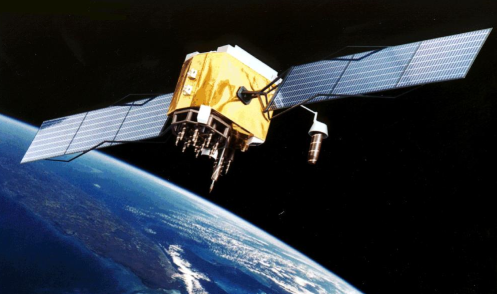
\includegraphics[keepaspectratio,height=5cm]{./Imagenes/06.00.navegacion/GPS-Satellite-IIF.png}
  \label{fig:satelite-GPS}}
  \subfigure[Sat\'elite GLONASS]{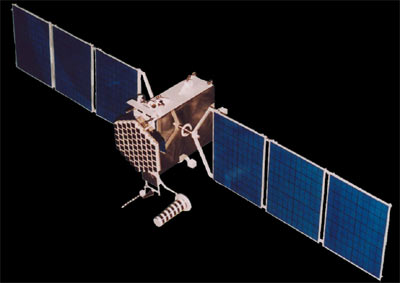
\includegraphics[keepaspectratio,height=5cm]{./Imagenes/06.00.navegacion/glonass.jpg}
  \label{fig:satelite-GPS}}
  \subfigure[Sat\'elite GALILEO]{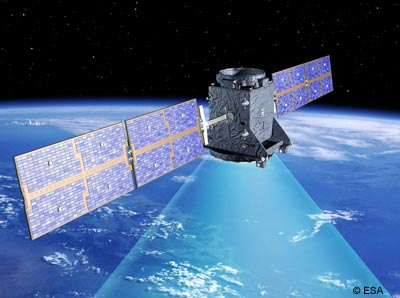
\includegraphics[keepaspectratio,height=5cm]{./Imagenes/06.00.navegacion/gps-galileo.jpg}
  \label{fig:satelite-GPS}}
  \caption{Navegaci\'on por sat\'elite}
\end{figure}

Es muy importante acotar que en la actualidad ninguno de los sistemas GNSS operativos pueden utilizarse, por s\'i solo, como m\'etodo \'unico de navegaci\'on a\'erea. Hay varias causas para esto:

\begin{itemize}
\item  Tanto el sistema GPS como el GLONASS son de
  naturaleza militar y no hay garant\'ia de que operen continuamente
  para los usuarios civiles (GALILEO se encuentra aun en fase de
  desarrollo).

\item  Ninguno de los sistemas GNSS proporciona,  actualmente, integridad. Es decir, la garant\'ia de que el piloto
  recibir\'a r\'apidamente y de manera autom\'atica la advertencia de que el
  sistema tiene una falla y dej\'o de funcionar adecuadamente.

\item  No hay garantia o cobertura de fiabilidad prove\'ida por sus operadores (e.g. accidentes aereos)
\item La fiabilidad es incierta en regiones de altas latitudes del norte de Europa
\item La precisi\'on es moderada para aplicaciones que requieren una r\'apida determinaci\'on de la posici\'on
\item A los usuarios no se les informa inmediatamente de los errores que ocurren en el sistema
\end{itemize}

Es por esta raz\'on que se han desarrollado sistemas adicionales a los GNSS que los complementan. \'Estos son los llamados \textbf{Sistemas de Aumento} y existen b\'asicamente tres categor\'ias:


\begin{description}
\item [SBAS] Sistemas de aumento basados en sat\'elites. Proporcionan sat\'elites auxiliares y estaciones de referencia en tierra con funciones espec\'ificas que complementan a los GNSS y los hacen aptos
  para navegaci\'on en ruta y aproximaciones a la pista. Los ejemplos
  son WAAS (estadunidense), EGNOS (europeo) y MSAS (japon\'es).

\item [GBAS] Sistemas de aumento basados s\'olo en instalaciones en
  tierra. El ejemplo t\'ipico es el LAAS (a\'un en desarrollo), son de
  corto alcance y est\'an enfocados en la asistencia en el aterrizaje.

\item [ABAS] Sistemas de aumento basados en instrumentos a bordo de la
  aeronave. Combinan informaci\'on de varios instrumentos aeron\'auticos y
  en funci\'on de esto monitorizan el estado de los sat\'elites GNSS.
\end{description}


\section{M\'etodos para determinar la posici\'on \cite{Salazar_nav_aerea}}

Adicionalmente al m\'etodo dead reckoning,  existen varias maneras de obtener la posici\'on seg\'un la naturaleza de las ayudas de navegaci\'on disponibles para el aeronavegante. 


\subsection{M\'etodo $\theta-\theta$}

Este m\'etodo se utiliza cuando se tienen disponibles varias radioayudas de tipo azimutal, o en general, cuando el sistema de navegaci\'on obtiene \'angulos entre ejes de referencia, puntos de referencia y la posici\'on actual.

Para explicar los fundamentos del m\'etodo, se debe imaginar que el sistema de navegaci\'on de la aeronave obtiene el \'angulo $\theta_1$ entre la posici\'on de la aeronave, el punto de referencia $P_1$ y un eje de referencia, tal y como ilustra la Figura \ref{fig:theta-fix}. Si el punto de referencia es, por ejemplo, una estaci\'on VOR, el eje de referencia apunta al norte magn\'etico. 

El conocimiento del \'angulo $\theta_1$ determina una l\'inea de posici\'on (o LOP, por sus siglas en ingl\'es). Se sabe entonces que la aeronave se encuentra en alg\'un lugar a lo largo de $LOP_{1}$: la l\'inea que empieza en el punto $P_1$ y se aleja de dicho punto en la direcci\'on $\theta_1$.

Si se toma un marco de referencia rectangular de origen cualquiera, con su eje $Y$ paralelo al el eje de referencia hacia el norte de la radioayuda, y se supone que las coordenadas del punto $P_1$ en dicho sistema vienen dadas por $(x_1, y_1)$, entonces se tiene una situaci\'on como la mostrada en la Figura\ref{fig:theta-lop1}. 

\begin{figure}[!h]
  \centering
 \subfigure[M\'etodo $\theta$]{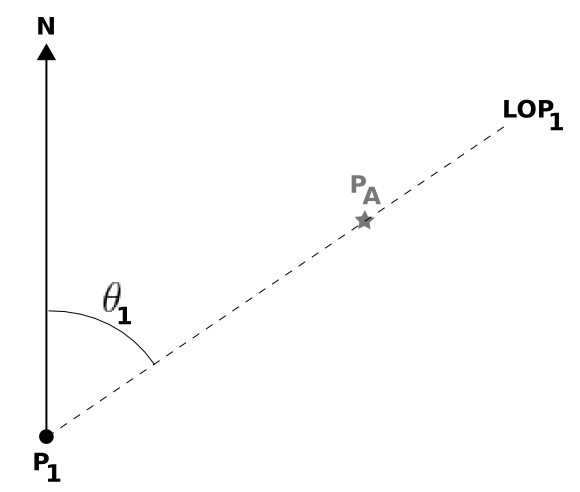
\includegraphics[width=0.45\textwidth]{./Imagenes/06.00.navegacion/theta-fix.png}  \label{fig:theta-fix}}
\subfigure[M\'etodo $\theta$ con marco de referencia ]{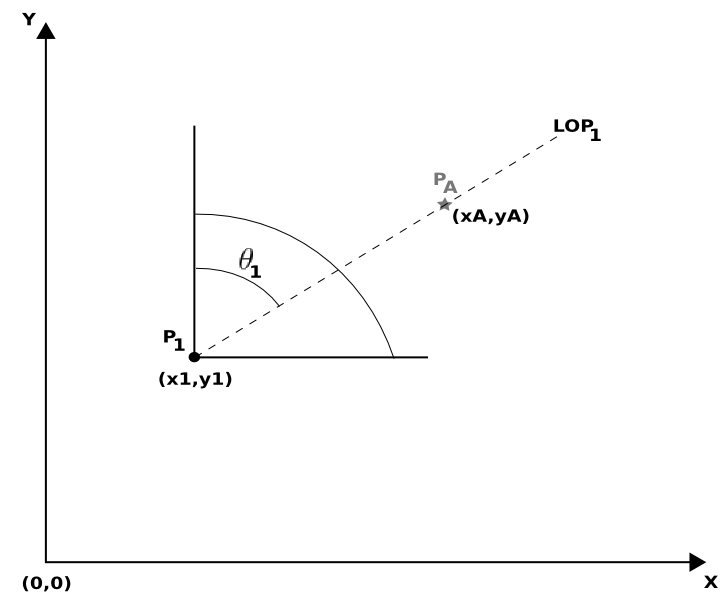
\includegraphics[width=0.45\textwidth]{./Imagenes/06.00.navegacion/theta-lop1.png}  \label{fig:theta-lop1}}
  \caption{M\'etodo $\theta-\theta$}
\end{figure}

Entonces, se puede demostrar que la posici\'on $(x_A, y_A)$ de la aeronave es posible expresarla de manera simple como la ecuaci\'on de una recta:


\begin{equation}\label{eq:metodo-theta}
 y_A = \tan (90-\theta_1) (x_A-x_1) + y_1
 \end{equation}





Sin embargo esta informaci\'on, aunque muy \'util, es insuficiente para determinar la posici\'on exacta de la aeronave: existe un n\'umero infinito de posiciones que cumple con la condici\'on establecida por la $LOP_{1}$ (Ecuaci\'on \ref{eq:metodo-theta}). Est\'a claro que se tiene una \'unica ecuaci\'on y que existen dos inc\'ognitas

Es por ello que se dice que hay una ambigüedad en la posici\'on. Para resolverla, es necesario obtener informaci\'on adicional. Hablando en t\'erminos matem\'aticos, es necesario encontrar otra ecuaci\'on que no sea linealmente dependiente de la primera.

Ahora bien, si dentro del alcance del sistema de navegaci\'on de la aeronave se encuentra otra estaci\'on VOR $P_2$ que proporcione una segunda medici\'on $\theta_2$, la situaci\'on ser\'a la planteada en la Figura \ref{fig:Theta-theta-fix}.

\begin{figure}[!h]
  \centering
  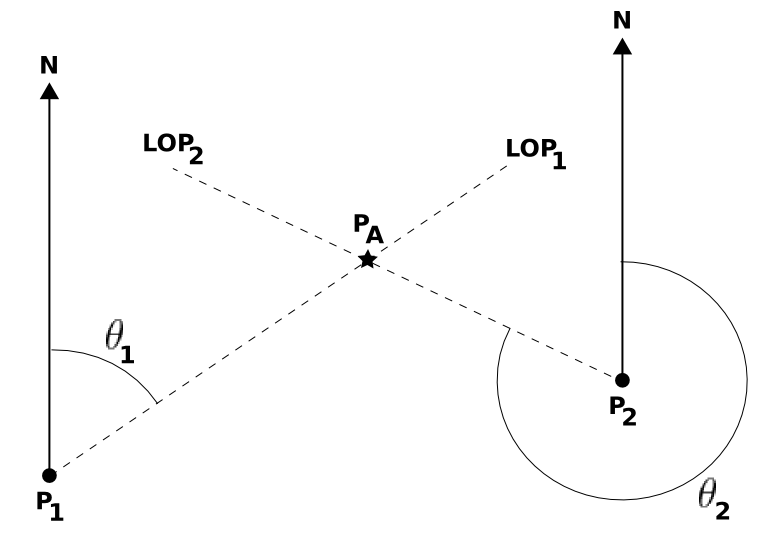
\includegraphics[width=0.5\textwidth]{./Imagenes/06.00.navegacion/theta-theta-fix.png}
  \caption{Theta-theta fix}
  \label{fig:Theta-theta-fix}
\end{figure}

En este caso, se tiene una segunda l\'inea de posici\'on $LOP_2$, que al intersectarse con $LOP_1$ proporcionar\'a la posici\'on de la aeronave. La Ecuaci\'on (\ref  {eq:theta-theta-fix}) representa a $LOP_2$.

\begin{equation}
  \label{eq:theta-theta-fix}
 y_A = \tan (90-\theta_2) (x_A-x_2) + y_2   
\end{equation}


Las Ecuaciones (\ref{eq:metodo-theta}) y (\ref  {eq:theta-theta-fix}) se combinan entonces para resolver el sistema y obtener la posici\'on.

Obviamente, en las consideraciones anteriores se ha supuesto que las coordenadas de los puntos $P_1$ y $P_2$ eran conocidas (de all\'i que se les considere puntos de referencia). Por lo general, esto supone que dichos puntos est\'an en lugares fijos. No obstante, pudiera darse el caso de que dichos puntos fueran m\'oviles, y entonces el sistema de navegaci\'on deber\'ia tener informaci\'on suficiente para calcular la posici\'on de los puntos de referencia en cada instante (como se hace, por ejemplo, con los sat\'elites de los sistemas GNSS). 

\subsection{M\'etodo $\theta-\rho$}

En ocasiones, junto con el VOR puede existir una estaci\'on DME colocalizada1.4 en el punto $P_1$. En este caso, adem\'as de un \'angulo $\theta_1$ se tiene una distancia o rango $\rho_1$, como indica la Figura \ref{fig:theta-rho-fix}.

\begin{figure}[!h]
  \centering
  \subfigure[M\'etodo $\theta-\rho$]{
     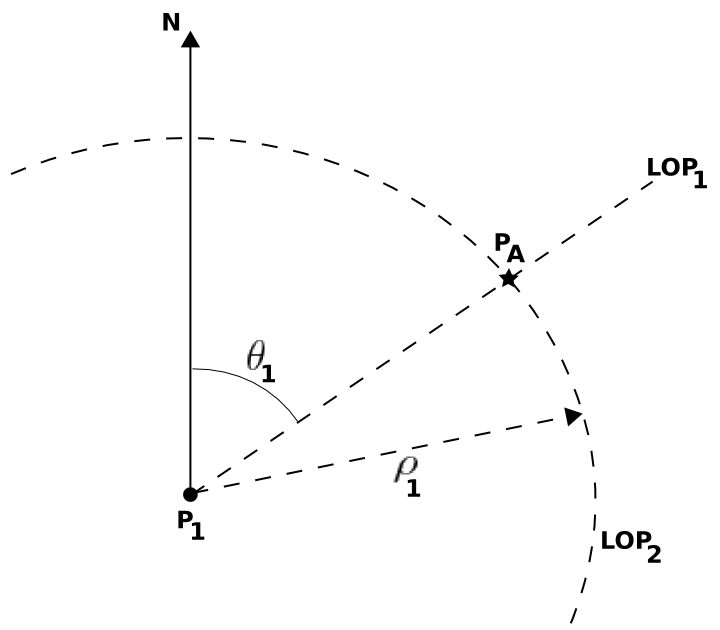
\includegraphics[height=6cm]{./Imagenes/06.00.navegacion/theta-rho-fix.png}  
     \label{fig:theta-rho-fix}
   }
  \subfigure[M\'etodo $\rho$-$\rho$]{
  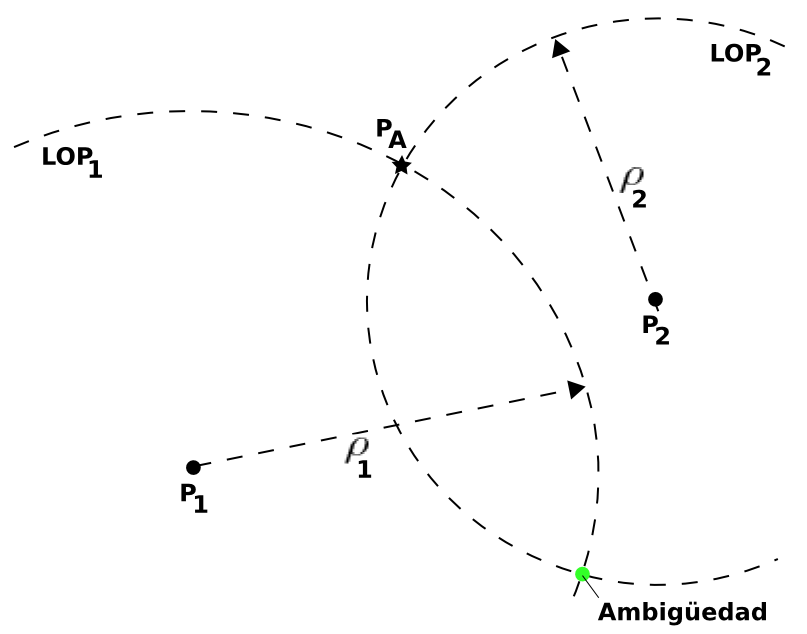
\includegraphics[height=6cm]{./Imagenes/06.00.navegacion/rho-rho-fix.png} 
  \label{fig:rho-rho-fix}
  }
  \caption{M\'etodos de navegaci\'on}
\end{figure}


Como puede verse, hay dos l\'ineas de posici\'on: $LOP_1$ correspondiente al \'angulo $\theta_1$ y $LOP_2$, que corresponde al rango $\rho_1$ (de hecho, est\'a ``\textit{l\'inea de posici\'on}'' es en realidad una circunferencia, pero el concepto se mantiene). En la intersecci\'on entre ambas LOPs se encuentra la aeronave.

La ecuaci\'on que corresponde a $LOP_2$ se puede expresar como:


\[ (y_A - y_1)^2 + (x_A - x_1)^2 = \rho_{1}^{2} \]

Note que este sistema puede resolverse incluso si el VOR y el DME no est\'an en el mismo lugar. Asimismo, es posible que la LOP de $\rho$ constante intersecte a la LOP de $\theta$ constante en m\'as de un lugar, dando como resultado una ambigüedad que deba resolverse con informaci\'on adicional. 


\subsection{M\'etodo $\rho$-$\rho$}

En este caso, se tienen al menos dos radioayudas que proporcionan informaci\'on de distancia, como se indica en la Figura \ref{fig:rho-rho-fix}

Se puede ver con facilidad la aparici\'on de una ambigüedad en la parte inferior de la Figura \ref{fig:rho-rho-fix}. Las fuentes de informaci\'on adicional usadas habitualmente para resolver dicha ambigüedad son:

\begin{itemize}\item  Agregar mediciones (ecuaciones) adicionales (de $\rho$ o $\theta$)
  que permitan discernir la posici\'on correcta.

\item Dado que la aeronave despega de una posici\'on conocida, un registro
  cuidadoso de la ruta seguida puede permitir discriminar cu\'al es la
  posici\'on correcta. Esto significa que se est\'a utilizando informaci\'on
  adicional del pasado (en vez del presente) para resolver la
  ambigüedad.

\item Para veh\'iculos terrestres y acu\'aticos, a veces es posible utilizar
  informaci\'on sobre el entorno para resolver la ambigüedad. Por
  ejemplo, el sistema de navegaci\'on de un barco puede descartar una
  ambigüedad que caiga en tierra, y el de un coche podr\'ia eliminar
  todas las posiciones posibles que caigan fuera de calles y
  carreteras.
\end{itemize}

\subsection{M\'etodo hiperb\'olico}

El m\'etodo hiperb\'olico es una versi\'on del $\rho$-$\rho$, pero en vez de utilizar los rangos absolutos se utiliza la diferencia entre ellos. Variaciones del m\'etodo usan la diferencia entre fases, o tiempos de recepci\'on, como muestran los diversos sistemas de navegaci\'on que utilizaban este m\'etodo, como el Omega, el LORAN, el Decca, etc.

El uso de la diferencia entre rangos genera LOPs que son hip\'erbolas, como muestra la Figura \ref{fig:metodo-hiperbolico}.

\begin{figure}[!h]
  \centering
  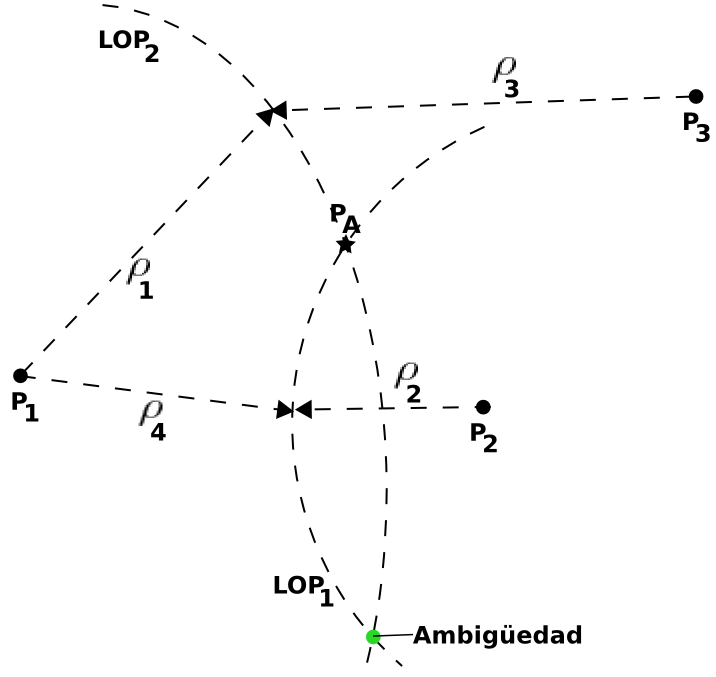
\includegraphics[width=0.5\textwidth]{./Imagenes/06.00.navegacion/hiperbolic-fix.png}
  \caption{M\'etodo hiperb\'olico}
  \label{fig:metodo-hiperbolico}
\end{figure}

Note que en la Figura  \ref{fig:metodo-hiperbolico} la ambigüedad queda resuelta al generar la hip\'erbola entre los puntos $P_2$ y $P_3$. 


\section{La Tierra}
\label{sec:la.tierra}

\subsection{Forma, tama\~no y movimientos}
\label{sec:forma.y.tamanio}

Desde el punto de la navegaci\'on, el planeta Tierra se considera una esfera perfecta, aunque en la realidad no lo sea. Inspecciones detalladas de su superficie han determinado variaciones en altura de, aproximadamente, 19 km desde el fondo del oc\'eano hasta el v\'ertice de la monta\~na m\'as alta, Figura \ref{fig:forma.tierra}.

Medida en el ecuador, el di\'ametro de la Tierra es aproximadamente $12756.274$\,km, mientras que el di\'ametro polar es de $12713.505$\,km. La diferencia entre estos di\'ametros es de $42.769$\,km y, este valor, puede ser utilizado para expresar la elipticidad de la Tierra (Figuras \ref{fig:dimensiones.tierra} y \ref{fig:amanecer.de.la.tierra}). El radio entre esta diferencia y el di\'ametro ecuatorial es:

\[\displaystyle
	\text{Elipticidad} = \frac{42.769 \,\text{m}}{ 12756.274\,\text{m}}
	=\frac{1}{298.257}
\]

\begin{figure}[!h]
  \centering

\subfigure[Forma de la tierra, dimensiones exageradas]{
	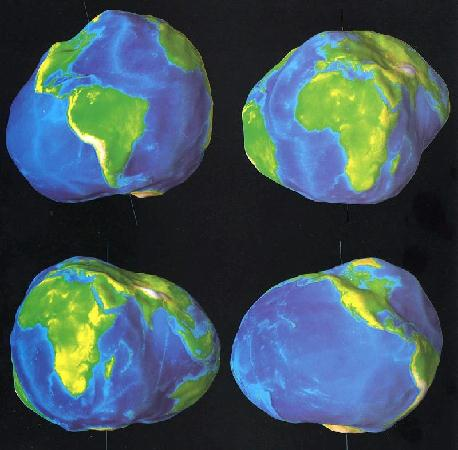
\includegraphics[height=6cm]{Imagenes/06.00.navegacion/forma-tierra.jpg}
	\label{fig:forma.tierra}}
  \subfigure[Amanecer de la Tierra, misi\'on \mbox{Apolo 8} (1968)]{
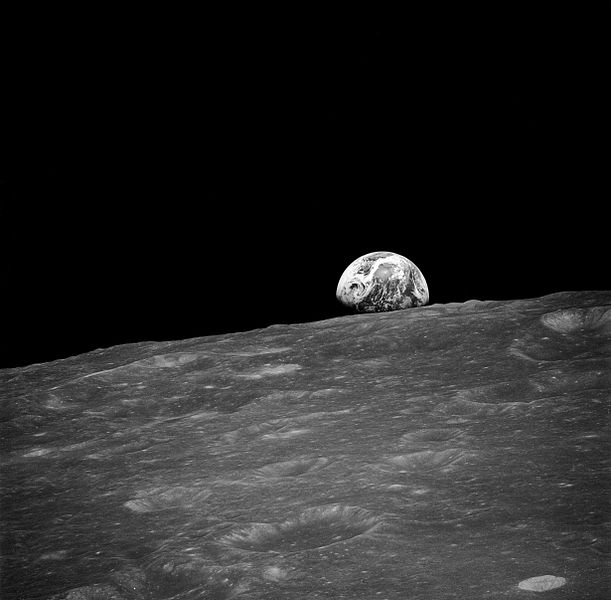
\includegraphics[height=6cm]{Imagenes/06.00.navegacion/amanecer-tierra.jpg}
 \label{fig:amanecer.de.la.tierra}}

  \subfigure[Dimensiones
%\\ {\tiny (Fuente: \url{http://www.kalipedia.com/geografia-general/tema/forma-dimensiones-tierra.html?x=20070417klpgeogra_6.Kes\&ap=1})}}
]{
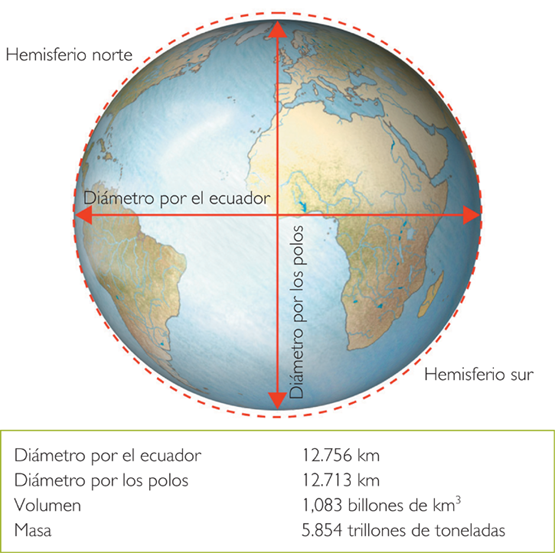
\includegraphics[height=6.5cm]{Imagenes/06.00.navegacion/dimensiones-tierra.png}
	  \label{fig:dimensiones.tierra}}
  \subfigure[
Rotaci\'on
]{
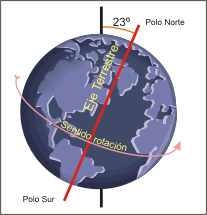
\includegraphics[height=6.5cm]{Imagenes/06.00.navegacion/RotacionTerrestre.png}
 \label{fig:rotacion.tierra}}
  \subfigure[
Precesi\'on
]{
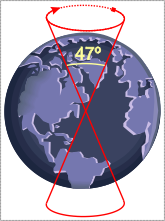
\includegraphics[height=6.5cm]{Imagenes/06.00.navegacion/Precesion.png}
 \label{fig:precesion.tierra}}
  \subfigure[
Nutaci\'on
]{
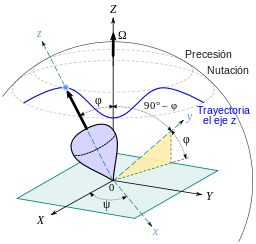
\includegraphics[height=6.5cm]{Imagenes/06.00.navegacion/nutacion.png}
 \label{fig:nutacion.tierra}}
  \subfigure[
Los movimientos \mbox{principales}
]{
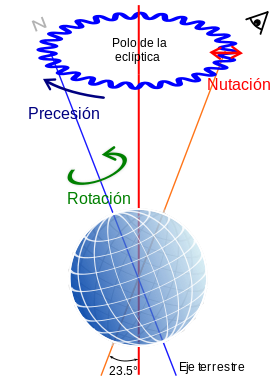
\includegraphics[height=6.5cm]{Imagenes/06.00.navegacion/rotacion-precession-nutation.png}
 \label{fig:los.tres.movimientos.tierra}}

  \caption{La Tierra}
\end{figure}

Dado que el di\'ametro ecuatorial excede al polar en 1 parte sobre 298, se considera que la Tierra es, pr\'acticamente, esf\'erica. 

La Tierra tiene los siguientes movimientos al desplazarse en el espacio:

\begin{itemize}
	\item \textbf{Movimiento de rotaci\'on:} Es un movimiento que efectúa la Tierra girando sobre sí misma a lo largo de un eje ideal denominado Eje terrestre que pasa por sus polos. Una vuelta completa, tomando como referencia a las estrellas, dura 23 horas con 56 minutos y 4 segundos y se denomina día sidéreo. Si tomamos como referencia al Sol, el mismo meridiano pasa frente a nuestra estrella cada 24 horas, llamado día solar. Los 3 minutos y 56 segundos de diferencia se deben a que en ese plazo de tiempo la Tierra ha avanzado en su órbita y debe de girar algo más que un día sideral para completar un día solar, Figura \ref{fig:rotacion.tierra}.

La primera referencia tomada por el hombre fue el Sol, cuyo movimiento aparente, originado en la rotación de la Tierra, determina el día y la noche, dando la impresión que el cielo gira alrededor del planeta. En el uso coloquial del lenguaje se utiliza la palabra día para designar este fenómeno, que en astronomía se refiere como día solar y se corresponde con el tiempo solar.

El eje terrestre forma un ángulo de 23,5º respecto a la normal de la eclíptica, fenómeno denominado oblicuidad de la eclíptica. Esta inclinación produce largos meses de luz y oscuridad en los polos geográficos, además de ser la causa de las estaciones del año, causadas por el cambio del ángulo de incidencia de la radiación solar.

        \item \textbf{Movimiento de traslación:} Es un movimiento por el cual la Tierra se mueve alrededor del Sol. La causa de este movimiento es la acción de la gravedad, originándose cambios que, al igual que el día, permiten la medición del tiempo. Tomando como referencia el Sol, resulta lo que se denomina año tropical, lapso necesario para que se repitan las estaciones del año. Dura 365 días, 5 horas y 47 minutos. El movimiento que describe es una trayectoria elíptica de 930 millones de kilómetros, a una distancia media del Sol de prácticamente 150 millones de kilómetros ó 1 U.A. (Unidad Astronómica). De esto se deduce que la Tierra se desplaza con una rapidez media de 106200 km/h (29,5 km/s).

La trayectoria u órbita terrestre es elíptica. El Sol ocupa uno de los focos de la elipse y, debido a la excentricidad de la órbita, la distancia entre el Sol y la Tierra varía a lo largo del año. A primeros días de enero se alcanza la máxima proximidad al Sol, produciéndose el perihelio, donde la distancia es de 147,5 millones de km,; mientras que en los primeros días de julio se alcanza la máxima lejanía, denominado afelio, donde la distancia es de 152,6 millones de km.

\item \textbf{Movimiento de precesión:} 
también denominado precesión de los equinoccios, es debido a que la Tierra no es esférica, sino un elipsoide achatado por los polos. Si la Tierra fuera totalmente esférica, sólo realizaría los movimientos anteriormente descritos, Figura \ref{fig:precesion.tierra}.

Una vuelta completa de precesión dura 25767 años, ciclo que se denomina año platónico, cuya duración había sido estimada por los antiguos mayas.

\item \textbf{Movimiento de nutación:} debido al achatamiento de los polos y a la atracción de la Luna sobre el eje ecuatorial. También en un movimiento de vaivén y se produce durante el movimiento de precesión, este recorre a su vez una pequeña elipse (como si fuese una pequeña vibración). Una vuelta completa a la elipse suponen 18,6 años, lo que supone que en una vuelta completa de precesión la Tierra habrá realizado 1385 bucles, Figura \ref{fig:nutacion.tierra}.

\item \textbf{Bamboleo de Chandler:} pequeña oscilación del eje de rotación de la tierra que añade 0,7 segundos de arco en un período de 433 días a la precesión de los equinoccios. Fue descubierto por el astrónomo norteamericano Seth Carlo Chandler en 1891, y actualmente no se conocen las causas que lo producen, aunque se han propuesto varias teorías (fluctuaciones climáticas causantes de cambios en la distribución de la masa atmosférica, posibles movimientos geofísicos bajo la corteza terrestre, etc.)


\end{itemize}


\subsection{Coordenadas geogr\'aficas}

El sistema de coordenadas geogr\'aficas determina todas las posiciones de la superficie terrestre utilizando las dos coordenadas angulares de un sistema de coordenadas esf\'ericas que est\'a alineado con el eje de rotaci\'on de la Tierra. Este define dos \'angulos medidos desde el centro de la Tierra:

\begin{itemize}
\item {\bf\Gls{latitud}:} mide el \'angulo entre cualquier punto y el ecuador. Las
  l\'ineas de latitud se llaman paralelos y son c\'irculos paralelos al
  ecuador en la superficie de la Tierra.

  La insolaci\'on terrestre depende de la latitud. Dada la distancia que
  nos separa del Sol, los rayos luminosos que llegan hasta nosotros
  son pr\'acticamente paralelos. la inclinaci\'on con que estos rayos
  inciden sobre la superficie de la Tierra es, pues, variable seg\'un la
  latitud. En la zona intertropical, a mediod\'ia, caen casi verticales,
  mientras que inciden tanto m\'as inclinados cuanto m\'as se asciende en
  latitud, es decir cuanto m\'as nos acercamos a los Polos. As\'i se
  explica el contraste entre las regiones polares, muy fr\'ias y las
  tropicales, muy c\'alidas.


\item {\bf \Gls{longitud}:} mide el \'angulo a lo largo del ecuador desde cualquier   punto de la Tierra. Se acepta que Greenwich en Londres es la
  longitud 0 en la mayor\'ia de las sociedades modernas. Las l\'ineas de
  longitud son c\'irculos m\'aximos que pasan por los polos y se llaman
  meridianos.
\end{itemize}


Combinando estos dos \'angulos, se puede expresar la posici\'on de cualquier punto de la superficie de la Tierra. Por ejemplo, El Cairo, en Egipto, tiene latitud 30 grados norte, y longitud 31 grados este. As\'i un vector dibujado desde el centro de la tierra al punto 30 grados norte del ecuador y 31 grados al este de Greenwich pasar\'a por El Cairo.

El ecuador es un elemento importante de este sistema de coordenadas; representa el cero de los \'angulos de latitud y el punto medio entre los polos. Es el plano fundamental del sistema de coordenadas geogr\'aficas.

\begin{figure}[!h]
  \centering
  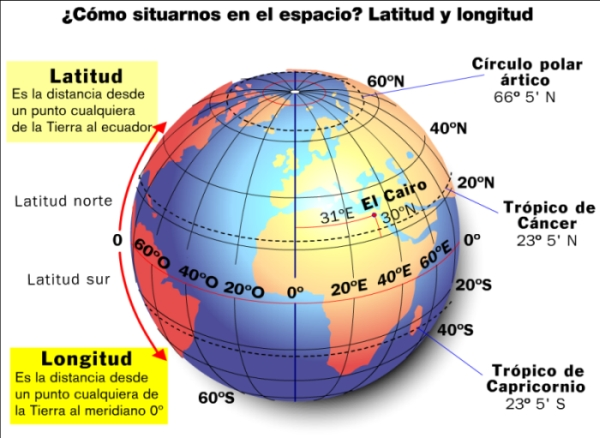
\includegraphics[width=\textwidth]{./Imagenes/06.00.navegacion/latitud_longitud.jpg}
  \caption{Latitud y longitud}
  \label{fig:latitud-longitud}
\end{figure}

El \textbf{Sistema de Coordenadas Universal Transversal de Mercator} (Universal Transverse Mercator, UTM) est\'a basado en un tipo de \gls{proyeccion-cartografica} denominada \emph{proyecci\'on geogr\'afica transversal de Mercator}, tangente a un meridiano. Las magnitudes en el sistema UTM se expresan en metros al nivel del mar, que es la base de la proyecci\'on del elipsoide de referencia.

El sistema de coordenadas UTM fue desarrollado por el Cuerpo de Ingenieros del Ejército de los Estados Unidos en la década de 1940. El sistema se basó en un modelo elipsoidal de la Tierra. Se usó el elipsoide de Clarke de 1866 para el territorio de los 48 estados contiguos. Para el resto del mundo –incluidos Alaska y Hawái– se usó el Elipsoide Internacional. Actualmente se usa el elipsoide WGS84 como modelo de base para el sistema de coordenadas UTM.

Anteriormente al desarrollo del sistema de coordenadas UTM varios países europeos ya habían experimentado la utilidad de mapas cuadriculados, en proyección conforme, al cartografiar sus territorios en el período de entreguerras. El cálculo de distancias entre dos puntos con esos mapas sobre el terreno se hacía más fácil usando el teorema de Pitágoras, al contrario que con las fórmulas trigonométricas que había que emplear con los mapas referenciados en longitud y latitud. En los años de post-guerra estos conceptos se extendieron al sistema de coordenadas basado en las proyecciones Universal Transversa de Mercator y Estereográfica Polar Universal, que es un sistema cartográfico mundial basado en cuadrícula recta.

La proyección transversa de Mercator es una variante de la proyección de Mercator que fue desarrollada por el geógrafo flamenco Gerardus Mercator en 1569. Esta proyección es conforme, es decir, que conserva los ángulos y casi no distorsiona las formas pero inevitablemente sí lo hace con distancias y áreas. El sistema UTM implica el uso de escalas no lineales para las coordenadas X e Y (longitud y latitud cartográficas) para asegurar que el mapa proyectado resulte conforme.

\begin{figure}[!htb]
  \centering
  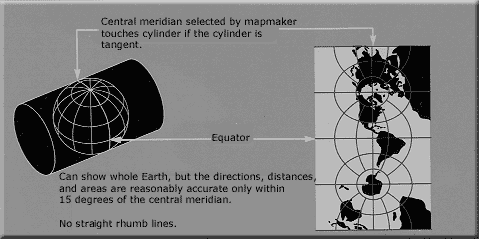
\includegraphics[width=\textwidth]{./Imagenes/06.00.navegacion/Usgs_map_traverse_mercator.png}
  \caption{Sistema de proyecci\'on transversa Mercator}
  \label{fig:sistema.proyeccion.transversa.mercator}
\end{figure}

La UTM es una proyección cilíndrica conforme. El factor de escala en la dirección del paralelo y en la dirección del meridiano son iguales (h = k). Las líneas loxodrómicas se representan como líneas rectas sobre el mapa. Los meridianos se proyectan sobre el plano con una separación proporcional a la del modelo, así hay equidistancia entre ellos. Sin embargo los paralelos se van separando a medida que nos alejamos del Ecuador, por lo que al llegar al polo las deformaciones serán infinitas. Por eso sólo se representa la región entre los paralelos 84ºN y 80ºS. Además es una proyección compuesta; la esfera se representa en trozos, no entera. Para ello se divide la Tierra en husos de 6º de longitud cada uno, mediante el artificio de Tyson .

La proyección UTM tiene la ventaja de que ningún punto está demasiado alejado del meridiano central de su zona, por lo que las distorsiones son pequeñas. Pero esto se consigue al coste de la discontinuidad: un punto en el límite de la zona se proyecta en coordenadas distintas propias de cada Huso.

Para evitar estas discontinuidades, a veces se extienden las zonas, para que el meridiano tangente sea el mismo. Esto permite mapas continuos casi compatibles con los estándar. Sin embargo, en los límites de esas zonas, las distorsiones son mayores que en las zonas estándar.

\begin{itemize}
	\item \textbf{  Husos UTM:}  Se divide la Tierra en 60 husos de 6º de longitud, la zona de
  proyección de la UTM se define entre los paralelos 80º S y 84º
  N. Cada huso se numera con un número entre el 1 y el 60, estando el
  primer huso limitado entre las longitudes 180° y 174° W y centrado
  en el meridiano 177º W. Cada huso tiene asignado un meridiano
  central, que es donde se sitúa el origen de coordenadas, junto con
  el ecuador. Los husos se numeran en orden ascendente hacia el
  este. Por ejemplo, la Península Ibérica está situada en los husos
  29, 30 y 31, y Canarias está situada en el huso 28. En el sistema de
  coordenadas geográfico las longitudes se representan
  tradicionalmente con valores que van desde los -180º hasta casi 180º
  (intervalo -180º → 0º → 180º); el valor de longitud 180º se
  corresponde con el valor -180º, pues ambos son el mismo

\item \textbf{Bandas UTM:}  Se divide la Tierra en 20 bandas de 8º Grados de Latitud, que se
  denominan con letras desde la C hasta la X excluyendo las letras "I"
  y "O", por su parecido con los números uno (1) y cero (0),
  respectivamente. Puesto que es un sistema norteamericano
  (estadounidense), tampoco se utiliza la letra "Ñ". La zona C
  coincide con el intervalo de latitudes que va desde 80º Sur (o -80º
  latitud) hasta 72º S (o -72º latitud). Las bandas polares no están
  consideradas en este sistema de referencia. Para definir un punto en
  cualquiera de los polos, se usa el sistema de coordenadas UPS. Si
  una banda tiene una letra igual o mayor que la N, la banda está en
  el hemisferio norte, mientras que está en el sur si su letra es
  menor que la "N".  

\item \textbf{Notación:} Cada cuadrícula UTM se define mediante el número del huso y la letra
  de la zona; por ejemplo, la Plaza España en la ciudad de C\'ordoba (Argentina) se encuentra en las coordenadas:
  \begin{itemize}
  \item latitud:31º 25' 43.38"  S
  \item longitud:64º 11' 5.84"  W
  \end{itemize}
  las cuales corresponden a las UTM 20J (6523614, 387522), ver Figura \ref{fig:zonas.utm}.  

\item \textbf{Excepciones:}  La rejilla es regular salvo en 2 zonas, ambas en el hemisferio
  norte; la primera es la zona 32V, que contiene el suroeste de
  Noruega; esta zona fue extendida para que abarcase también la costa
  occidental de este país, a costa de la zona 31V, que fue
  acortada. La segunda excepción se encuentra aún más al norte, en la
  zona que se conoce como Svalbard (ver mapa para notar las
  diferencias).
\end{itemize}


\begin{figure}[!htb]
  \centering
  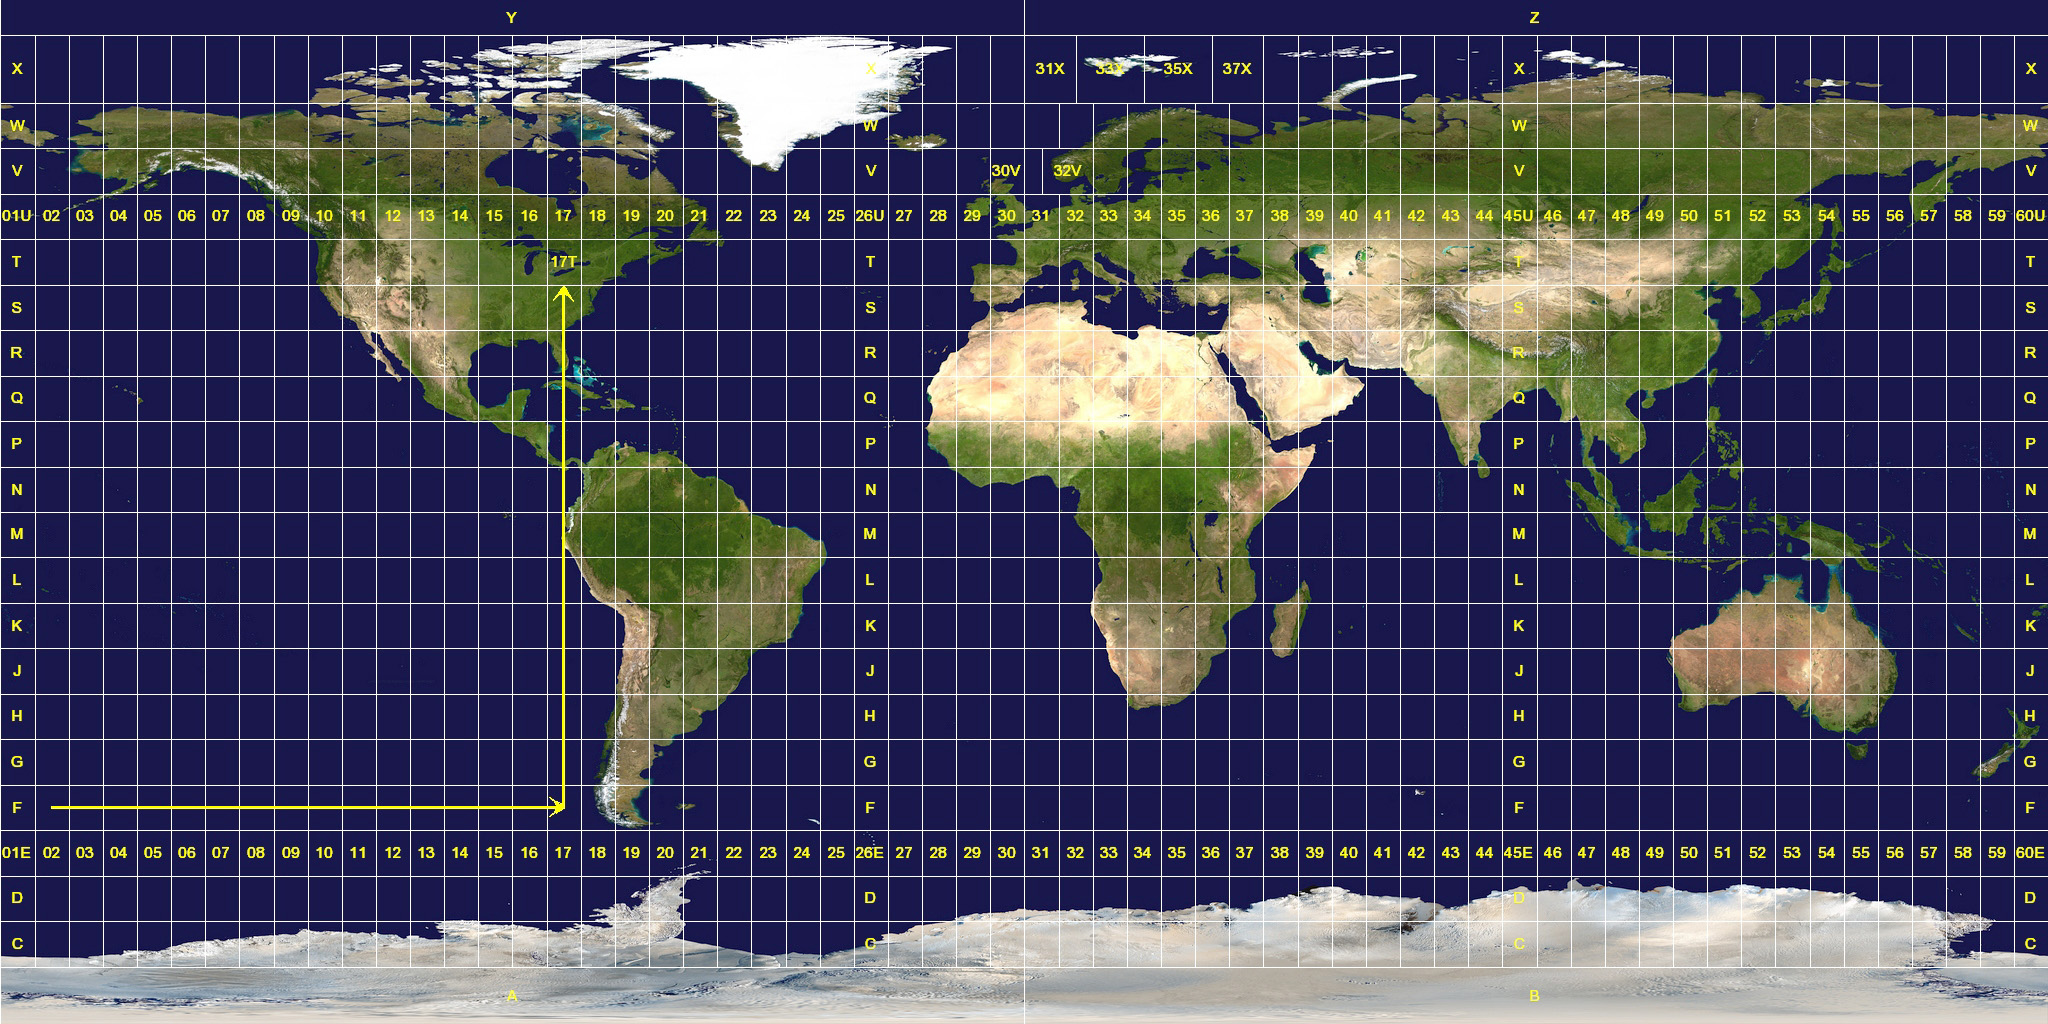
\includegraphics[width=\textwidth]{./Imagenes/06.00.navegacion/Utm-zones.jpg}
  \caption{Zonas UTM}
  \label{fig:zonas.utm}
\end{figure}


\section{Distancia, direcci\'on, tiempo, el Norte}
\label{sec:distancia.direccion.tiempo}

\subsection{Distancia}
\label{sec:distancia}

La distancia se mide como la longitud de la l\'inea que une a dos puntos, su unidad habitual para el uso en navegaci\'on es la \emph{\gls{nauticalmile}} (NM), la cual se define como 1 minuto de latitud o $6076$\,pies ($1852$\,m). A veces es necesario convertir de NM a \gls{statutemile} (SM) y viceversa, lo cual se hace de la siguiente forma:

\[\displaystyle
	\frac{\text{Millas estatutarias}}{\text{Millas n\'auticas}} 
	= \frac{76}{66}
\]

Relacionado con el concepto de distancia se encuentra el de \emph{velocidad}, el cual indica la tasa de cambio de posici\'on. La velocidad se expresa usualmente en millas por hora (mph). Si la medida de la distancia es en NM, entonces la velocidad se expresa en \gls{nudo}. Una velocidad de 200 nudos es igual a una velocidad de 200 NM por hora.

Para calcular la distancia entre puntos sobre la superficie terrestre es necesario tener en cuenta no es plana, lo que implica que existir\'an ligeras (o grandes) distorsiones si se realiza esta operaci\'on sobre un mapa (dependiendo
del tipo de este ultimo).
  
Adem\'as, el hecho de que la Tierra sea un geoide introduce variaciones
adicionales, que deber\'an  (o no) tenerse en cuenta dependiendo de la precisi\'on con que se desee realizar la medici\'on. 

A los fines de una primera aproximaci\'on, puede asumirse que la Tierra es esf\'erica.

Entre dos puntos cualesquiera de la superficie terrestre pueden trazarse líneas curvas diferentes: la ortodrómica, la loxodrómica. %y la isoazimutal.

\begin{description}
\item[Loxodr\'omica \label{loxodromica}]  (del griego   \greektext lox'oc
  % λοξóς
  \latintext ``oblicuo'' y \greektext dr'omoc
  % δρóμος
  \latintext  ``carrera, curso'') a la línea que une dos puntos cualesquiera de la
  superficie terrestre cortando a todos los meridianos con el mismo
  ángulo, ver Figura \ref{fig:loxodromica}. La loxodrómica, por tanto, es fácil de seguir manteniendo el
  mismo rumbo marcado por la brújula. Su representación en el mapa
  dependerá del tipo de proyección del mismo, por ejemplo en la de
  Mercator es una recta.

\item[Ortodrómica \label{ortodromica}] (del griego \greektext enje'ia 
\latintext ``recto'' y
\greektext dr'omoc
 \latintext ''carrera'') es el camino más corto entre dos puntos de la superficie terrestre; es el arco del círculo máximo que los une, menor de 180 grados, Figura \ref{fig:ortodromica}. 

% \item[Isoazimutal] La línea o curva isoazimutal, IsoZ($X,\theta$), es el lugar geométrico de los puntos sobre la superficie terrestre cuyo rumbo inicial ortodrómico respecto a un punto fijo $X$ es constante e igual a $\theta$.

% Es decir, si el rumbo inicial ortodrómico desde S hasta X es de 80 grados, la línea isoazimutal asociada es la formada por todos los puntos cuyo rumbo ortodrómico inicial al punto X es de 80º.
\end{description}

\begin{figure}[!h]
  \subfigure[Loxodr\'omica]{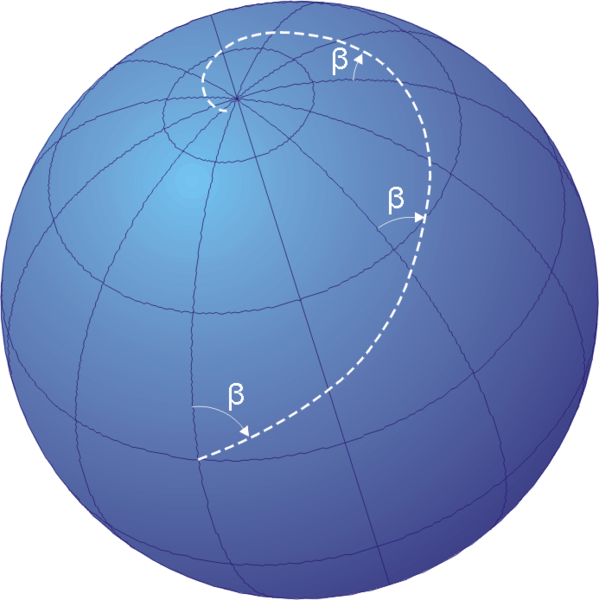
\includegraphics[height=5.8cm]{./Imagenes/06.00.navegacion/loxodromica.png} \label{fig:loxodromica}}
  \subfigure[Ortodr\'omica]{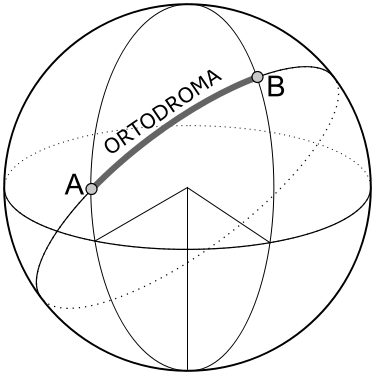
\includegraphics[height=5.8cm]{./Imagenes/06.00.navegacion/ortodroma.png} \label{fig:ortodromica}}
  \subfigure[Comparaci\'on de ambas l\'ineas]{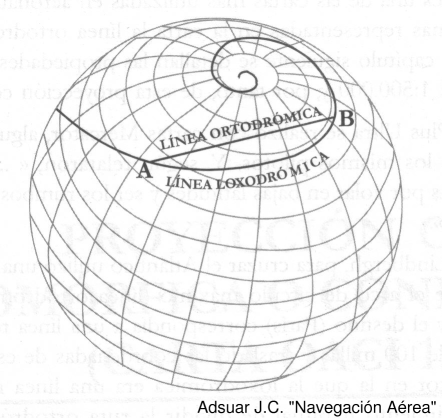
\includegraphics[height=5.8cm]{./Imagenes/06.00.navegacion/comp-loxo-orto.png} \label{fig:ortodromica.loxodromica.comparacion}}
	\caption{Distancia entre dos puntos sobre la Tierra}
\end{figure}

Pedro Nunes, un geógrafo portugués, publicó en Tratado de la navegación (1546) un descubrimiento con grandes implicaciones para la navegación. Antes de él se creía que, marchando sobre la superficie terrestre con un rumbo fijo, es decir, formando un ángulo constante con la meridiana, la línea recorrida era un círculo máximo. Dicho con otras palabras, que un navío que siguiese este derrotero daría la vuelta al mundo y volvería al punto de partida. Nunes señaló la falsedad de este concepto al demostrar que la curva recorrida se va acercando al polo, alrededor del cual da infinitas vueltas, sin llegar nunca a él; o, dicho en lenguaje técnico, que tiene el polo por punto asintótico.

Una característica de la ortodrómica es que presenta un ángulo diferente con cada meridiano, (excepto cuando dicha ortodrómica coincide con un meridiano o con el ecuador). Esta característica representó un grave inconveniente para la navegación, solucionado hacia los últimos años del Siglo XX con el sistema GPS, porque antes del mismo, era difícil trazar una ruta de navegación que siguiera la ortodrómica ya que obligaría a continuos cambios de rumbo. Cuando las distancias eran grandes y seguir el camino más corto suponía un ahorro significativo, se realizaba una aproximación marcando una serie de puntos intermedios, en los cuales se cambiaba de rumbo, y de ésta manera se lograba una aproximación a las correspondientes loxodrómicas.

\subsection{Direcci\'on}
\label{sec:direccion}

La direcci\'on es la posici\'on de un punto en el espacio relativo a otro sin referencia a la distancia entre ellos. En la navegaci\'on se utiliza un sistema n\'umerico para indicar la direcci\'on como el mostrado en la Figura \ref{fig:rosa.de.compas}. En la misma se divide la vista en planta en 360º, comenzando con el norte a 000º y continuando en sentido de las agujas del reloj, pasando por el este a 90º, sur 180º y oeste 270º, volviendo al norte.

Este c\'irculo se denomina rosa de comp\'as, las l\'ineas cuasi-verticales de la Figura \ref{fig:rosa.de.compas} son meridianos. Por el punto A pasa el meridiano a trav\'es de 000º y 180º de la rosa, el punto B se encuentra en una direcci\'on de 60º respecto del A y el punto C en una direcci\'on de 220º del punto A.

\subsubsection{Definiciones}
\label{sec:definiciones.navegacion}

\begin{description}

\item [Trayectoria] (trayectory) se define como el conjunto de puntos del espacio por los cuales pasa la aeronave durante su vuelo (ver Figura \ref{fig:trayectoria}).

\item [Ruta] es la curva resultante de proyectar la trayectoria sobre la superficie de la Tierra (ver Figura \ref{fig:trayectoria}).

\item [Waypoints] son puntos conocidos a lo largo de la ruta, y a menudo resaltan por alguna raz\'on en particular (Lugares de reporte obligatorio, puntos de intersecci\'on de aerov\'ias, etc.) (ver Figura \ref{fig:trayectoria}).

\item [Tramo] (leg) se define como un segmento de ruta comprendido entre dos waypoints (ver Figura \ref{fig:trayectoria}). 

\begin{figure}[!h]
  \centering
  \subfigure[Rosa de comp\'as]{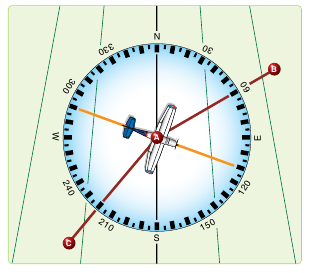
\includegraphics[height=6.7cm]{./Imagenes/06.00.navegacion/rosa.png}  \label{fig:rosa.de.compas}}
  \subfigure[Trayectoria, ruta]{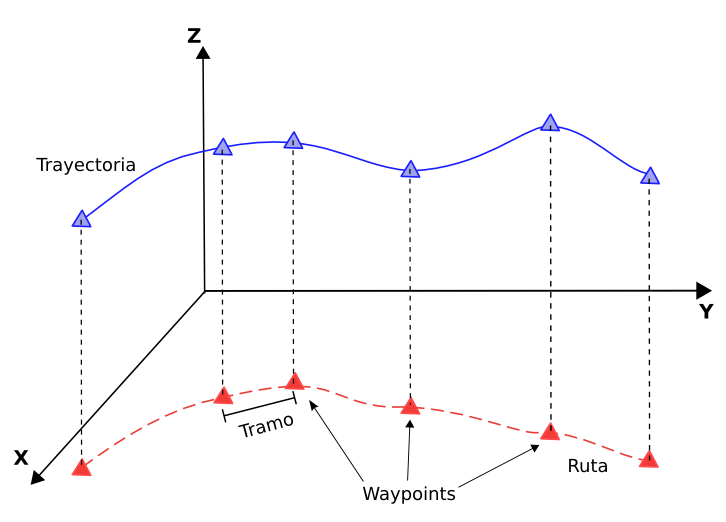
\includegraphics[height=6.7cm]{./Imagenes/06.00.navegacion/trayectoria-ruta.png}  \label{fig:trayectoria}} 

  \caption{Elementos de navegaci\'on}
\end{figure}


  \item[Rumbo] el rumbo o o ``Heading'' (HDG) es el \'angulo entre el norte y el eje   longitudinal de la aeronave (hacia donde apunta su nariz). No
  coincide necesariamente con el vector velocidad (Track) dado que es
  posible, por ejemplo, que el piloto modifique el rumbo para
  contrarestar un viento cruzado (ver Figura \ref{fig:curso}).

\item [Curso deseado] es el \'angulo entre el norte (cualquiera que se est\'e usando: magn\'etico, geogr\'afico, etc) y la l\'inea recta que une dos waypoints sucesivos en la ruta. En ingl\'es se denomina ``\textit{Desired Track}'', y se abrevia DTK (ver Figura \ref{fig:curso}).

\item [Derrota] En n\'autica, la derrota es el trayecto que ha recorrido una embarcaci\'on desde un punto ``\textit{A}'' hasta otro punto ``\textit{B}''. En el derrotero o carta n\'autica se traza la ruta a seguir; contiene informaciones importantes para el navegante, tales como ubicaci\'on de faros, boyas, profundidad del agua, etc. En navegaci\'on a\'erea es el \'angulo entre el norte y la l\'inea tangente a la ruta (dicha tangente corresponde, por cierto, al vector velocidad de la aeronave). En ingl\'es se le llama ``\textit{Track}'' o TK (ver Figura \ref{fig:curso}).

\item [Error transversal] El error transversal o ``\textit{Cross-Track Error}'' (XTE) es la distancia perpendicular entre la posici\'on de la aeronave y la l\'inea que representa al curso deseado. \footnote{Es conveniente tener en cuenta que la diferencia entre el curso deseado (DTK) y la ruta realmente seguida (TK) por lo general es producida por factores externos tales como el viento cruzado (en el caso de las aeronaves) o las corrientes marinas (si se habla de barcos).}

\end{description}

\begin{figure}[!h]
  \centering
  \subfigure[Curso]{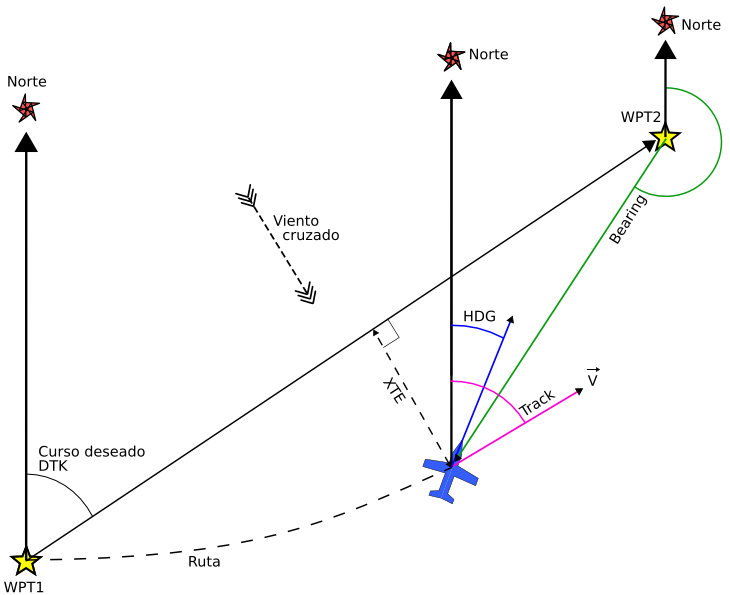
\includegraphics[keepaspectratio,height=10cm]{./Imagenes/06.00.navegacion/curso-derrota-rumbo-marcacion.png}  \label{fig:curso}}
  \caption{Elementos de navegaci\'on (continuaci\'on)}
\end{figure}

\subsection{Tiempo}
\label{sec:tiempo}

La navegaci\'on a\'erea es un problema de cuatro dimensiones: latitud, longitud, altura y es necesario saber \emph{en qu\'e momento} estuvimos (o estaremos) en una posici\'on dada.

Muchos de los sistemas de navegaci\'on modernos est\'an basados en la medici\'on de intervalos de tiempo.

La medici\'on del tiempo se encuentra asociada a la historia del calendario, esto es, un modo sistem\'atico de organizar los d\'ias en semanas, meses, a\~nos y milenios.

Una de las formas m\'as sencillas es con referencia a las fases de la Luna, el calendario de este tipo es denominado \emph{lunar} y el tiempo entre repeticiones de una fase dada de la Luna (p.e., luna nueva) es denominado \emph{mes sin\'odico}. Este dura, en promedio, $29.530589$ d\'ias.

El calendario lunar tiene como ventaja que posee una referencia muy f\'acil de seguir, pero tiene como inconveniente que el mes sin\'odico no tiene un n\'umero entero de d\'ias.

Por otra parte, las estaciones del a\~no son fen\'omenos muy importantes para la vida humana, pero las fases de la Luna son independientes de estas. Por ese motivo algunas culturas prefirieron marcar el paso del tiempo siguiendo el movimiento aparente del Sol por el cielo (ecl\'iptica\footnote{El movimiento que realiza la Tierra en torno al Sol (traslación), genera un plano al que se le ha dado el nombre de Eclíptica. Como el eje de giro de la Tierra tiene una inclinación promedio de 23° 27', entonces el Ecuador terrestre y la eclíptica forma entre si, este mismo ángulo.\\La proyección de la Eclíptica sobre la Esfera Celeste, forma un círculo máximo que se encuentra inclinado con respecto a ella, 23° 27'.
\\ La incidencia perpendicular de los haces de luz solar, barren casi 47º (exactamente 46º 54´) sobre el globo terráqueo. Cuando inciden a 23º 27´ Latitud Norte, alcanzan el denominado Trópico de Cáncer (21 de Junio). Cuando inciden a 23º 27´ Latitud Sur, el Trópico de Capricornio. Estos son los puntos máximos y mínimos que alcanzará el Sol en su desplazamiento imaginario por el cielo. Estos puntos reciben el nombre de Solsticios, del latín Solstitium, que significan “el Sol más lejos”. Los nombres de los Trópicos están determinados por las constelaciones de Cáncer, en el Hemisferio Norte del la Esfera Celeste y de Capricornio, en el Sur.
\\ De manera similar, existen dos puntos en donde se interceptan el Ecuador Celeste y la Eclíptica. Estos son el Punto Vernal  ubicado en la constelación de Los Peces (Piscis) y el Punto Otoñal (d) ubicado en la constelación de La Virgen (Virgo). El Punto Vernal representa en las coordenadas celestes lo que el Meridiano de Greenwich en las coordenadas terrestres, es decir el punto origen de las coordenadas celestes.
\\ En estos dos puntos, los haces de luz solar inciden perpendicularmente sobre el Ecuador de la Tierra, iluminando de manera uniforme a todo el planeta. Estos puntos reciben el nombre de Equinoccios, del latín Aequus Nox, que significa “igual duración de las noches”. En su recorrido anual, la Tierra alcanza estos puntos el 21 de marzo y 21 de Septiembre, respectivamente. }
). Este calendario se denomina \emph{solar}, y el tiempo transcurrido entre dos pasos suscesivos del Sol por el equinoccio de primavera es denominado \emph{a~no vernal equinoxial} y tiene una duraci\'on de $365.2424$ d\'ias.

Se comprob\'o que  19 a\~nos vernales equinoxiales equivalen a $234.997$ meses sin\'odicos ($\approx 235$), lo que implica que cada 19 a\~nos las fases de la Luna y sus fen\'omenos asociados (eclipses) caen casi ex\'actamente en la misma fecha. Este ciclo es denominado \emph{met\'onico} en honor al astr\'onomo Met\'on, siglo V a. C.

Posteriormente los romanos establecieron un calendario que, tras sucesivas adaptaciones, evolucion\'o al calendario actualmente utilizado en el hemisferio occidental, el calendario Gregoriano.

La medici\'on del tiempo tiene, actualmente, dos familias:
\begin{itemize}
\item Las asociadas al movimiento de los cuerpos celestes
\item Las basadas en las oscilaciones de los \'atomos
\end{itemize}

\subsubsection{Tiempo solar}
\label{sec:tiempo.solar}

El tiempo solar es una medida del tiempo fundamentada en el movimiento aparente del Sol sobre el horizonte del lugar. Toma como origen el instante en el cual el Sol pasa por el Meridiano, que es su punto más alto en el cielo, denominado mediodía.1 A partir de este instante se van contando las horas en intervalos de 24 partes hasta que completan el ciclo diurno.

Sin embargo, el Sol no tiene un movimiento regular a lo largo del año, y por esta razón el tiempo solar se divide en dos categorías:

\begin{itemize}
\item {\bf Tiempo solar verdadero} está basado en el día solar verdadero,
  el cual es el intervalo entre dos regresos sucesivos del Sol al
  meridiano. Puede ser medido con un reloj de sol, y se corresponde
  con el amanecer, el mediodía o el anochecer: se basa en lo que es
  posible observar de manera directa. Con un reloj de sol adecuadamente orientado se puede marcar este tiempo, Figura \ref{fig:reloj.de.sol}.

La duración de un día solar verdadero varía a lo largo del año. Esto se debe a que la órbita terrestre es una elipse, con lo cual la Tierra en su movimiento de traslación se mueve más veloz cuando se acerca al Sol y más despacio cuando se aleja de él. Debido a esto, el día solar más corto es el 15 de septiembre, mientras que el día solar más largo es el 22 de diciembre, tanto el Hemisferio Norte como en el Hemisferio Sur.


\item \textbf{ Tiempo solar medio} está basado en un sol ficticio que viaja a una   velocidad constante a lo largo del año, y es la base para definir el
  día solar medio (24 horas u $86400$ segundos). Se corresponde con el
  tiempo civil y se coordina mediante el Tiempo Medio de Greenwich.
\end{itemize}


La diferencia entre el tiempo solar verdadero y el tiempo solar medio, que en ocasiones llega a ser de 15 minutos, es llamada \emph{Ecuación de tiempo}, Figura \ref{fig:2012.ecuacion.del.tiempo}.


\begin{figure}[!h]
  \centering
  \subfigure[Reloj de sol]{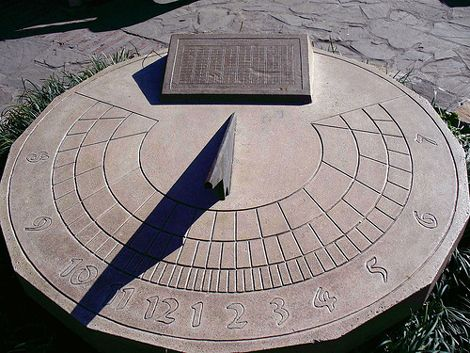
\includegraphics[height=6.5cm]{./Imagenes/06.00.navegacion/reloj-de-sol.jpg} \label{fig:reloj.de.sol}}
  \subfigure[Ecuaci\'on del tiempo, a\~no 2012]{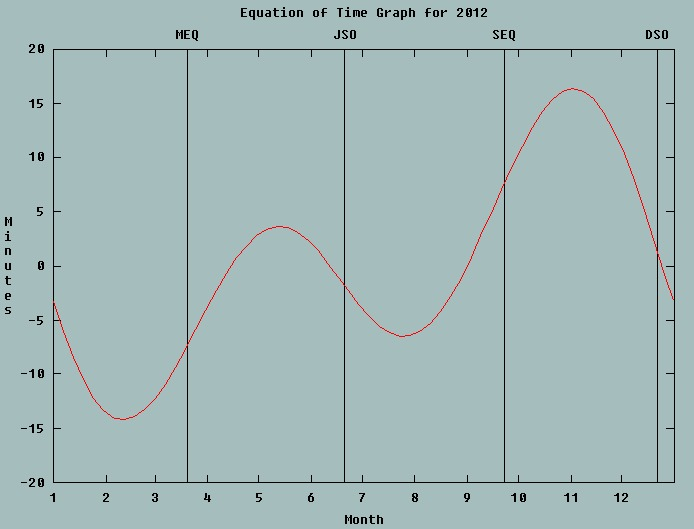
\includegraphics[height=6.5cm]{./Imagenes/06.00.navegacion/2012-ecuacion-tiempo.jpg} \label{fig:2012.ecuacion.del.tiempo}}

  \subfigure[Meridiano de Greenwich]{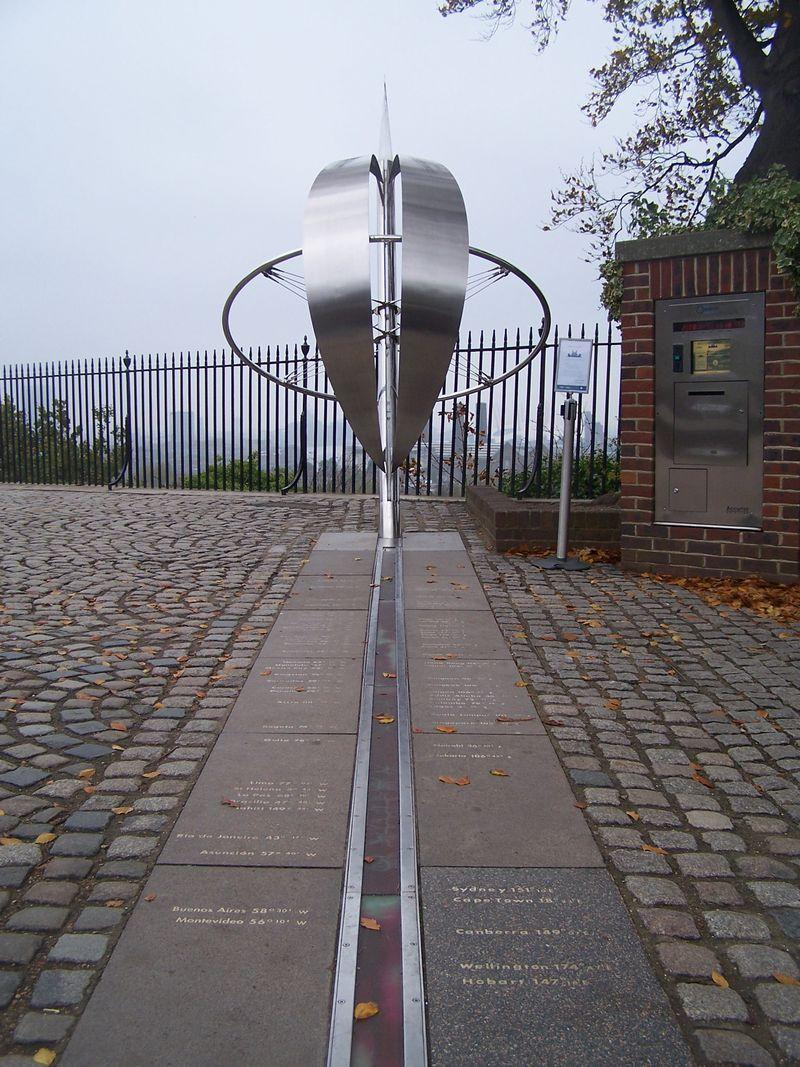
\includegraphics[height=6.5cm]{./Imagenes/06.00.navegacion/Greenwich-Meridian-Line.jpg} \label{fig:meridiano.greenwich}}
  \subfigure[Primer reloj at\'omico (1948)]{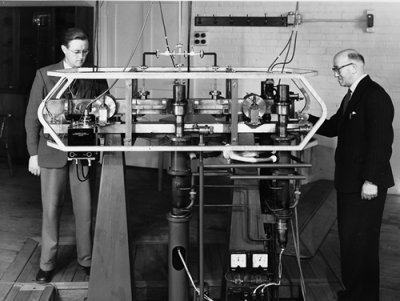
\includegraphics[height=6.5cm]{./Imagenes/06.00.navegacion/TAI.jpg} \label{fig:primer.reloj.atomico}}

  \caption{Medici\'on del tiempo}
\end{figure}

\subsubsection{ Greenwich Mean Time}
\label{sec:greenwich.mean.time}

El  Greenwich Mean Time (GMT)  es una escala de tiempo basada en el paso
del Sol Medio por el meridiano de Greenwich (espec\'ificamente por el viejo
Observatorio Real de Greenwich, que es el punto de referencia).
Este tiempo est\'a  obsoleto pues en 1928 la Uni\'on Astron\'omica 
 Internacional introdujo el  Universal Time (UT) para reemplazarlo.

\subsubsection{Tiempo Universal (UT)}
\label{sec:tiempo.universal}

El UT reemplaz\'o al GMT puesto que este \'ultimo se basaba en la medici\'on de la posici\'on del Sol, y existen problemas asociados a la medici\'on precisa de la misma.

El UT se basa en la medici\'on de la posici\'on de referencias astron\'omicas, como los cu\'asares, consigui\'endose mayor precisi\'on.

 A pesar de su mayor precisión el UT sigue siendo una escala de tiempo no uniforme, pues en el fondo se basa en la medición del período de rotación del planeta y éste presenta anomalías. De hecho, en 1956 el Comité Internacional de Pesos y Medidas decidió que la definición del segundo se haría en función del período de revolución de la Tierra para una época dada, y así el segundo de efemérides fue definido como:

La fracción 1/31556925,9747 del año tropical medio para el 1ro. de Enero de 1900 a las 12 horas.

Debido a la existencia de las mencionadas anomalías, existen varios tipos de UT:
\begin{description}

\item [UT0:] Es el Tiempo Universal definido mediante observaciones de
  puntos de referencia astronómicos. Inicialmente era medido mediante
  relojes de péndulo, pero conforme la tecnología de los relojes fue
  avanzando, se notó la existencia de errores.


\item [UT1:] Cuando a UT0 se le aplican las correcciones debidas al
  movimiento de los polos (efecto Chandler y otros) obtenemos
  UT1. Esta escala es la más ampliamente utilizada por los astrónomos
  y a menudo el término UT se refiere a ella.


\item [UT2:] Debido a que la velocidad de rotación de la Tierra no es
  constante, UT1 presenta variaciones estacionales relacionadas, entre
  otras cosas, a las mareas y el intercambio de energía entre la
  Tierra y la atmósfera. Al aplicar las correcciones debidas a las
  variaciones más fuertes y regulares (del orden de 3 milisegundos por
  día), obtenemos UT2. Esta escala, la más precisa para el Tiempo
  Universal, sigue siendo irregular y por ello ha caído en desuso
  después de la aparición de nuevos métodos no astronómicos para la
  medición del tiempo.
\end{description}


\subsubsection{ Temps Atomique International (TAI)}
\label{sec:temps.atomique.international}

 Dado que las escalas de tiempo anteriores no eran suficientemente regulares, se desarrollaron relojes cada vez más precisos que permitieron desligarse de la rotación de la Tierra como patrón que definía el tiempo. Estas investigaciones desembocaron en el reloj atómico, que marca el tiempo examinando el comportamiento de los átomos de un material dado, y por tanto la escala de tiempo así construida no depende (o depende muy poco) de factores externos.

Desde mediados de 1950 se empezaron a desarrollar relojes atómicos suficientemente precisos y por ello la 13ra. Conferencia General de Pesos y Medidas celebrada en el año 1967 pudo definir el segundo del Sistema Internacional como:

\vspace{3mm}

\fbox{\parbox{\textwidth}{La duración de 9192631770 períodos de la onda de la radiación emitida por el átomo de Cesio 133 cuando se realiza la transición entre los dos niveles hiperfinos del estado fundamental del átomo.}}

\vspace{3mm}

En función de esta definición, la BIPM (Oficina Internacional de Pesos y Medidas), localizada en París, Francia, coordina y promedia los datos provenientes de un gran número de relojes atómicos alrededor del globo para generar una escala de tiempo uniforme llamada TAI (Tiempo Atómico Internacional). 



\subsubsection{Tiempo Universal Coordinado (UTC)}
\label{sec:tiempo.universal.coordinado}
 El UTC es una escala de tiempo atómica internacional ampliamente utilizada en el ámbito civil. De hecho, hoy en día prácticamente todos los países del mundo definen sus horas locales en función de UTC6.9, añadiendo o restando un número entero de horas según convenga a su localización geográfica.

En cierta forma, UTC puede verse como la manera de reconciliar el tiempo atómico (TAI) con el tiempo dado por la rotación de la Tierra (Tiempo Universal \#1 - UT1).

UTC tiene la misma frecuencia del TAI pero cada cierto tiempo se le añaden (o sustraen) segundos extras (llamados ``leap seconds'') para mantenerlo sincronizado dentro de +/- 0,9 s de UT1. De esta manera, se obtiene la exactitud del tiempo atómico sin divorciarse completamente del fenómeno de la rotación terrestre.

Los ``leap seconds'' empezaron a usarse el 30 de Junio de 19726.10, y habitualmente se introducen al final del último minuto del último día de diciembre o del último día de junio, si hace falta. Hasta el momento6.11 se han introducido 33 s (todos ellos de retraso).

\subsubsection{Tiempo GPS (GPST)}
\label{sec:tiempo.gps}


También llamado GPST, el tiempo GPS es el utilizado como referencia para las aplicaciones relacionadas con el sistema de posicionamiento global por satélite del Departamento de Defensa de los EE.UU.

El GPST es un tiempo de naturaleza atómica que no es alterado por ``leap seconds''. Toma como época de origen las 00:00 UTC de la noche del 5 al 6 de enero de 1980. Dado que para esa fecha se habían introducido 19 ``leap seconds'', la siguiente expresión es válida:

TAI - GPST = 19 s

Un concepto adicional importante es la llamada semana GPS. Ésta empieza la noche del sábado al domingo, de modo tal que el 17 de marzo del 2004 correspondió a la semana GPS 1262. Las semanas GPS tienen un ciclo de 1024, y el primer ciclo se alcanzó en la noche del 21 al 22 de Agosto de 1999, llamado ``GPS Week Rollover''. 

\subsubsection{Tiempo Loran-C}
\label{sec:tiempo.loran.c}

%El término LORAN, que significa ``Long Range Navigation'' (Navegación de Largo Alcance), co\-rres\-pon\-de a una cadena de transmisores de radiofrecuencia de amplio alcance que permiten conocer con cierta precisión (aproximadamente 0,25 NM) la posición de un receptor sobre la superficie terrestre.

Los transmisores pertenecientes a la cadena (o ``chain'', en inglés) Loran poseen relojes atómicos que están sincronizados entre sí. Estos relojes no son alterados por ``leap seconds'', lo que hace que se separe progresivamente de UTC.

La época de inicio de los relojes atómicos del sistema Loran-C fue las 0h del 01/Ene/1958.

\subsection{El Norte}
\label{sec:el.norte}
El concepto de ``\emph{Norte}'' engloba una serie de definiciones que es necesario conocer y diferenciar adecuadamente:

\begin{itemize}
\item\textbf{ Norte geográfico: }Es el que viene dado por la intersección del eje de rotación de la Tierra con la superficie de la misma [1]. Es llamado también "Norte verdadero", y en él confluyen todos los meridianos.

\item \textbf{Norte magnético:} Es el punto donde la mayor parte de las líneas de fuerza del campo magnético terrestre entran en la superficie. Se puede detectar utilizando instrumentos tales como la brújula y la "flux valve" (equivalente a la brújula en las aeronaves modernas).

Es importante hacer notar que el norte geográfico y el magnético \textbf{NO} coinciden, y que además el norte magnético cambia su posición con el tiempo.

\item \textbf{Declinación magnética:} Es el ángulo de desviación entre las posiciones del norte magnético y geográfico, vistas desde un punto en particular. Se denota como D y se considera positiva cuando el ángulo medido está hacia el Este del norte verdadero, y negativo en caso contrario. 

Lo anterior significa que si sobre un punto de la superficie terrestre la brújula marca un rumbo de 115º, y sabemos que la declinación magnética en ese punto es 4º E, el rumbo verdadero serán 119º. 

En la Figura \ref{fig:declinacion-magnetica} se representa la declinación magnética para dos puntos diferentes de la superficie terrestre. Note que en uno de ellos la geometría es tal que la declinación es cero. 

\begin{figure}[!h]
    \centering
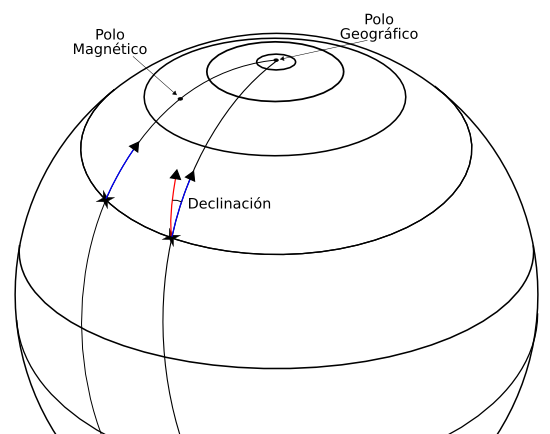
\includegraphics[keepaspectratio,width=0.6\textwidth]{./Imagenes/06.00.navegacion/declinacion-magnetica.png}
\caption{Declinaci\'on magn\'etica en dos puntos diferentes de la Tierra \cite{Salazar_nav_aerea}}
\label{fig:declinacion-magnetica}
\end{figure}

\item \textbf{Líneas isógonas:} Se llaman así a las líneas que, sobre las cartas de navegación o los mapas, unen puntos que tienen la misma declinación magnética. Son también denominadas Líneas Isogónicas. Adicionalmente, si una línea corresponde a puntos con declinación 0º, se habla de Línea Agónica. 

\item \textbf{Norte de la Brújula:} Es el norte magnético tal y como lo indica a bordo el instrumento adecuado (brújula o flux valve). No indica realmente el norte magnético pues el instrumento comete errores por diversas razones (presencia de masas metálicas cercanas, líneas de campo magnético que no son horizontales, etc).

\item \textbf{Desviación magnética:} Es el error angular cometido por la brújula o flux valve. El fabricante de la aeronave puede corregirla hasta cierto punto.

La Figura \ref{fig:declinacion-desviacion} presenta la relación entre los nortes geográfico, magnético y de la brújula con sus correspondientes diferencias angulares.

\begin{figure}[!htb]
    \centering
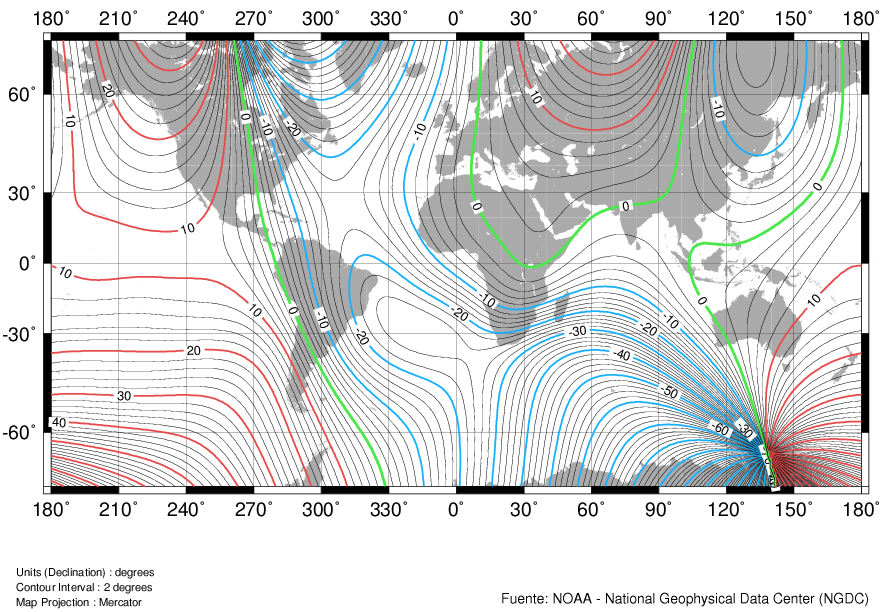
\includegraphics[keepaspectratio,width=\textwidth]{./Imagenes/06.00.navegacion/declinacion-magnetica-anio-2000.png}
\caption{Declinaci\'on magn\'etica - A\~no 2000 \cite{Salazar_nav_aerea}}
\label{fig:declinacion-magnetica-anio-2000}
\end{figure}

\begin{figure}[!htb]
    \centering
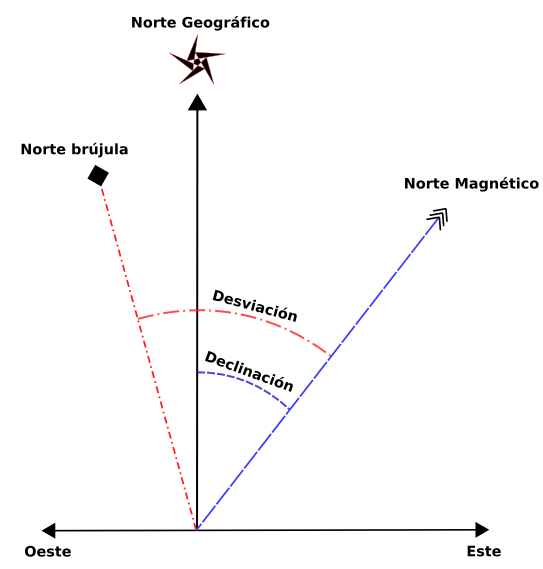
\includegraphics[keepaspectratio,width=0.6\textwidth]{./Imagenes/06.00.navegacion/declinacion-desviacion.png}
\caption{Los diferentes nortes y sus diferencias angulares \cite{Salazar_nav_aerea}}
\label{fig:declinacion-desviacion}
\end{figure}


\item \textbf{Norte de la Cuadrícula:} Cuando se navega a grandes latitudes (muy al norte o muy al sur del planeta), no tiene sentido guiarse por el norte magnético debido, entre otras cosas, a las grandes declinaciones implicadas.

Es por ello que se define arbitrariamente el Norte de la Cuadrícula como el norte indicado por los meridianos de la carta de navegación que se está usando para navegar. 
\end{itemize}





\section{Cartas de navegaci\'on aeron\'autica}
\label{sec:cartas.navegacion.aeronautica}

La carta aeron\'autica se define como la representaci\'on de una porci\'on de la tierra, su relieve y construcciones, dise\~nada especialmente para satisfacer los requisitos de la navegaci\'on a\'erea. Se trata de un mapa en el que se reflejan las rutas que deben seguir las aeronaves, y se facilitan las ayudas, los procedimientos y otros datos imprescindibles para el piloto.

El gran problema asociado a la construcción y utilización de cartas es que la superficie de la Tierra \textbf{no se puede representarse con fidelidad en ninguna carta}. Esto se debe a que una esfera \emph{no es una superficie desarrollable}, es decir, no es posible convertirla a un plano sin generar distorsiones. Es el mismo problema que enfrentaríamos si intentáramos convertir la cáscara de una naranja en un plano sin alterarla, Figura \ref{fig:comparacion.proyecciones.cartograficas}. 

Superficies que sí son desarrollables son los cilindros y los conos. En ambos casos, basta con cortar dichas superficies por un lugar conveniente y seguidamente las podemos estirar sin deformarlas y convertirlas en planos.

Por esta razón, la práctica común al construir una carta consiste en proyectar la superficie de la Tierra sobre una de estas tres superficies (plano, cono o cilindro). Dicha proyección consiste en escoger un conjunto de reglas geométricas y aplicarlas sistemáticamente a toda la superficie que se interesa proyectar, Figura \ref{fig:proyecciones.cartograficas}.

\subsection{Proyecciones cartogr\'aficas}
\label{sec:proyecciones.cartograficas}

Como las cartas de navegación en realidad son proyecciones de la superficie terrestre, es conveniente estudiar primero las características de las proyecciones para entender luego las de las cartas. 

 Existe un gran número de tipos diferentes de proyecciones según el conjunto de reglas que se escojan para hacerla (por ejemplo: punto de origen, tipo de superficie de proyección, posición de la superficie, etc.). Cada uno de estos conjuntos de reglas introduce diferentes tipos de distorsiones, que son inevitables, y en base a éstas se puede a su vez definir diferentes propiedades de la proyección.

\begin{figure}[!h]
  \centering
  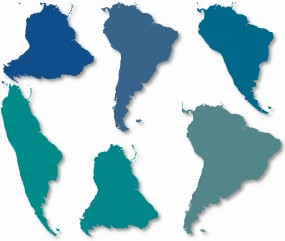
\includegraphics[width=0.8\textwidth]{./Imagenes/06.00.navegacion/comparacion-proyecciones.jpg}
  \caption{Am\'erica del Sur en diferentes proyecciones. ¿Cu\'al es la correcta? \\{\footnotesize Fuente: \url{http://www.progonos.com/furuti/MapProj/Normal/TOC/cartTOC.html}}}
  \label{fig:comparacion.proyecciones.cartograficas}
\end{figure}


La razón de que existan tantos tipos de proyecciones diferentes es que estas propiedades las hacen adecuadas para un uso u otro, según lo que se desee. En las siguientes secciones estudiaremos las propiedades más importantes que pueden tener las proyecciones, y por ende, las cartas hechas con ellas. 

\begin{figure}[!h]
  \centering
  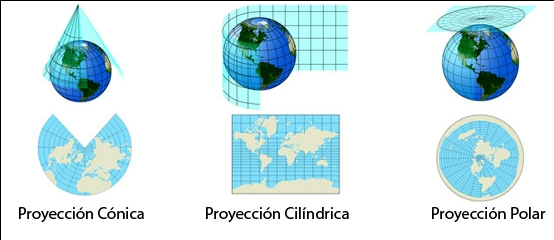
\includegraphics[width=\textwidth]{./Imagenes/06.00.navegacion/proyecciones.jpg}
  \caption{Proyecciones cartogr\'aficas}
  \label{fig:proyecciones.cartograficas}
\end{figure}

Entre las propiedades de las proyecciones se tiene:

\begin{description}
\item[Conformidad] Un mapa conforme es aquél que preserva los ángulos (y por tanto, las formas) a nivel local. Esto significa que las formas de características tales como deltas, ríos, etc. son reconocibles, pues la distorsión que sufren no es grande.
\item[Equivalencia] Una proyección es equivalente o autálica si mantiene las proporciones entre las áreas representadas. Esto quiere decir que si un país dado A tiene el doble del área que un país B, en una proyección equivalente dicha proporción se mantiene, Figura \ref{fig:groenlandia.africa.comparacion.superficies.segun.tipo.proyeccion}. 

Las proyecciones equivalentes o autálicas son de escasa utilidad para la navegación, pero por otra parte son muy útiles cuando se quiere presentar información que ha de compararse a simple vista, como población, producción industrial, etc., o para elaborar atlas escolares.


\begin{figure}[!h]
  \centering
  \subfigure[Proyeccion Mercator]{
  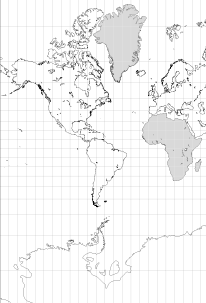
\includegraphics[height=7cm]{./Imagenes/06.00.navegacion/merEqTh.png}
  \label{fig:proyeccion.mercator.groenlandia.africa}
  }
  \subfigure[Proyeccion Mollweide]{
  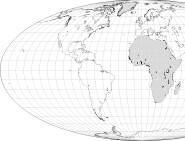
\includegraphics[height=7cm]{./Imagenes/06.00.navegacion/mollEqTh.png}
  \label{fig:proyeccion.mollweide.groenlandia.africa}
  }
  \caption{Comparaci\'on de las superficies de Groenlandia y \'Africa seg\'un el tipo de proyecci\'on utilizada, superficie \'Africa = 29800000\,km$^2$, superficie Groenlandia = 2175600\,km$^2$\\{\footnotesize Fuente: \url{http://www.progonos.com/furuti/MapProj/Normal/CartProp/AreaPres/areaPres.html}}
}
  \label{fig:groenlandia.africa.comparacion.superficies.segun.tipo.proyeccion}
\end{figure}


\item[Equidistancia] Una proyección es equidistante cuando posee un conjunto bien definido y completo de líneas a lo largo de las cuales la escala se mantiene constante, Figura \ref{fig:proyeccion.equidistante}.

Al indicar que posee un conjunto bien definido y completo de líneas, nos referimos al hecho de que muchas proyecciones tienen unas pocas líneas a lo largo de las cuales la escala se mantiene constante (a menudo llamadas líneas automecoicas. No obstante, en las cartas equidistantes el número de líneas que tienen esta propiedad es mucho más grande.

Por ejemplo, es posible crear una carta con una proyección equidistante que esté centrada en una ciudad dada A, y entonces se podría calcular con exactitud la distancia entre tal ciudad A y cualquier otra ciudad que se represente en la carta.

Las cartas equidistantes a menudo distorsionan mucho los ángulos y áreas, y por ello tienen una utilidad limitada. Sin embargo es posible obtener pocas distorsiones si el área representada es pequeña. 

    \begin{figure}[!h]
      \centering
  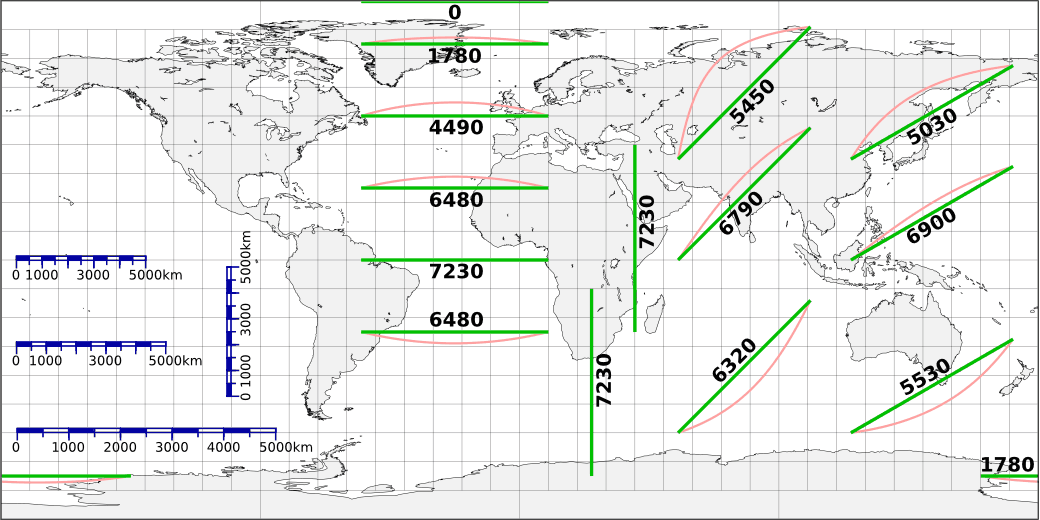
\includegraphics[height=9cm]{./Imagenes/06.00.navegacion/proyeccion-equidistante.png}
      \caption{Proyecci\'on equidistante cil\'indrica, distancias en km. Cada escala gr\'afica es v\'alida a lo largo de su propio paralelo. Solo la escala vertical es v\'alida en cualquier lugar.\\{\footnotesize Fuente: \url{http://www.progonos.com/furuti/MapProj/Normal/CartProp/AreaPres/areaPres.html}}}
      \label{fig:proyeccion.equidistante}
    \end{figure}


\item[Dirección]  Otra propiedad importante de las proyecciones es la referida a si distorsionan, y de qué manera, las direcciones. Por ejemplo, una proyección que muestra de forma correcta todas las direcciones desde su centro a cualquier otro punto de la carta se llama azimutal.

Hay al menos dos maneras diferentes de entender la dirección: En función del círculo máximo y en función del rumbo, y ambas maneras definen líneas muy importantes: 

\begin{description}
	\item[Líneas Loxodrómicas] ver  \fullref{loxodromica}
	\item[Líneas Ortodrómicas] ver \fullref{ortodromica}
\end{description}

En la Figura \ref{fig:comparacion.entre.loxodromas.y.ortodromas} puede observarse una comparaci\'on entre este tipo de l\'ineas al conectar dos puntos.

\begin{figure}[!h]
  \centering
  \subfigure[Proyecci\'on Mercator]{
	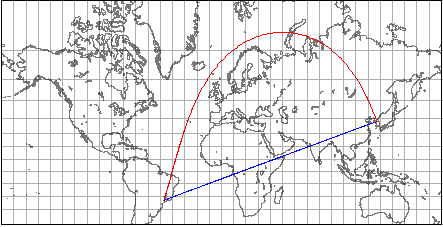
\includegraphics[height=6cm]{./Imagenes/06.00.navegacion/gr-mr-s70-n80-s-40.png}
	}
  \subfigure[Proyecci\'on polar azimutal equidistante]{
	\includegraphics[height=6cm]{./Imagenes/06.00.navegacion/gr-aze-s70.png}
	}
  \subfigure[Proyecci\'on Lagrange]{
	\includegraphics[height=6cm]{./Imagenes/06.00.navegacion/lg-s70h.png}
	}
  \caption{Comparaci\'on entre loxodromas y ortodromas, azul loxodromica, rojo ortodromica \\{\footnotesize Fuente: \url{http://www.progonos.com/furuti/MapProj/Normal/ShapePres/shapePres.html}}}
  \label{fig:comparacion.entre.loxodromas.y.ortodromas}
\end{figure}

\end{description}

\subsection{Las cartas OACI \cite{Salazar_nav_aerea}}

La seguridad de la navegaci\'on a\'erea exige la elaboraci\'on y publicaci\'on de cartas aeron\'auticas actualizadas y precisas, que respondan a las necesidades actuales de la aviaci\'on. En consecuencia, corresponde a cada Estado miembro de la Organizaci\'on de Aviaci\'on Civil Internacional (OACI) adoptar las disposiciones necesarias para facilitar el esfuerzo de cooperaci\'on que supone la producci\'on y difusi\'on de cartas aeron\'auticas. Adem\'as, cada Estado tiene la obligaci\'on de proporcionar informaci\'on del propio territorio a trav\'es de las cartas aeron\'auticas.

La Organizaci\'on de Aviaci\'on Civil Internacional (OACI), en su Anexo 4 - Cartas Aeron\'auticas, ha publicado una serie de normas y m\'etodos recomendados para la elaboraci\'on de las mismas. Adicionalmente, y como complemento y ayuda para la puesta en pr\'actica de estas normas, tambi\'en proporciona el Manual de Cartas Aer\'onauticas.

Seg\'un la OACI, el dise\~no de las cartas aeron\'auticas debe tomar en cuenta una serie de factores, entre los cuales se pueden mencionar:

\begin{itemize}

\item  Debe utilizarse una proyecci\'on com\'un.

  \item Las escalas utilizadas deben tener valores f\'acilmente
  comprensibles.

  \item Debe facilitarse la transici\'on de una carta a otra durante el
  vuelo mediante una adecuada selecci\'on de alturas, construcciones u
  otra informaci\'on relativa al terreno.

  \item Deber\'ian publicarse simult\'aneamente las cartas que tienen conexi\'on
  entre s\'i, ya sean cartas nuevas o sus revisiones.

\end{itemize}

\begin{landscape}
  \newcommand{\minitab}[2][1]{\begin{tabular}{#1}#2\end{tabular}}
Cartas opcionales. Las seis cartas opcionales se producir\'an si, en opinión de las Autoridades aeron\'auticas de los Estados, contribuyen a la seguridad, regularidad y eficacia de las operaciones de las aeronaves.

Cartas condicionales. Las cinco cartas condicionales se producir\'an solamente si se cumplen determinadas condiciones o circunstancias.

\begin{table}%[!h]
  \centering
  \caption{Cartas aeron\'auticas OACI}
  \label{tab:cartas.aeronauticas.OACI}
  \begin{small}
    \begin{tabular}{|m{0.12\textheight}|m{0.4\textheight}|c|c|c|m{0.35\textheight}|}
      \cline{3-5} 
	\multicolumn{2}{c|}{} & %\multirow{2}*[1.5cm]{
      \begin{turn}{90}
        \textbf{Obligatoria}
      \end{turn}
      % }
      &%\multirow{2}*[1.5cm]{
      \begin{turn}{90}
        \textbf{Opcional}
      \end{turn}
      % }
      &%\multirow{2}*[1.5cm]{
      \begin{turn}{90}
        \textbf{Condicional \,}
      \end{turn}
      % } 
      & \multicolumn{1}{c}{}
      \\ \cline{1-2}\cline{6-6}
      \centering \textbf{Grupo} & \centering \textbf{Carta} & 
      & & &\multicolumn{1}{c|}{\textbf{Requerimientos}}\\ \hline

      \multirow{4}{0.12\textheight}{ Planificaci\'on previa al vuelo} &
      \parbox{\linewidth}{1. Plano de obst\'aculos de aeródromo – Tipo A \\
      (limitadores de utilización).} 
	&\cellcolor{red} & & &
       Aeródromos con obst\'aculos destacados en las \'areas de despegue y aterrizaje.
	\\
&&&&& \\
&&&&& \\
&&&&& \\

%       \multirow{4}{0.12\textwidth}{ Planificaci\'on previa al vuelo} &
%       \minitab[l]{1. Plano de obst\'aculos de aeródromo – Tipo A \\
%       \quad (limitadores de utilización).} &\cellcolor{red} & & &
%        Aeródromos con obst\'aculos destacados en las \'areas de despegue y aterrizaje.
% 	\\
%       &
%       2. Plano de obst\'aculos de aeródromo – Tipo B. & &\cellcolor{blue} & & \\
%       &
%       3. Plano de obst\'aculos de aeródromo – Tipo C.& & &\cellcolor{green} & \\
%       &
%       4. Carta topogr\'afica para aproximaciones de precisión. &\cellcolor{red} & & & Obligatoria en pistas con aproximaciones de precisión categorías II y III\\ \hline
%       \multirow{4}{0.12\textwidth}{ En vuelo} &
%       5. Carta de navegación en ruta. &\cellcolor{red} & & & 
% 	Zonas en las que se hayan establecido Regiones de Información de Vuelo (FIR)	\\
%       &
%       6. Carta de \'area. & & &\cellcolor{green} & \\
%       &
%       7. Carta de salida normalizada – Vuelo por instrumentos (SID). & & &\cellcolor{green} & \\
%       &
%       8. Carta de llegada normalizada – Vuelo por instrumentos (STAR). & & &\cellcolor{green} & \\
%       &
%       9. Carta de aproximación por instrumentos. &\cellcolor{red} & & &
% Aeródromos en los que se haya establecido tal tipo de aproximación \\
%       &
%       10. Carta de aproximación visual.  & & &\cellcolor{green} & \\ \hline
%       \multirow{4}{0.12\textwidth}{Movimientos en tierra %de 
%         %	las aeronaves en el aeródromo
%       } &
%       11. Plano de aeródromo/helipuerto &\cellcolor{red} & & & 
% En todos los que se utiliza regularmente la aviación civil internacional\\
%       &
%       12. Plano de aeródromo para movimientos en tierra.  & &\cellcolor{blue} & & \\
%       &
%       13. Plano de estacionamiento y atraque de aeronaves.  & &\cellcolor{blue} & & \\ \hline
%       \multirow{4}{0.12\textwidth}{Navegación a\'erea visual, trazado de posiciones, planificación} &
%       14. Carta aeron\'autica mundial (escala 1:1.000.000). & \cellcolor{red}& & & En todas las zonas especificadas por la OACI\\
%       &
%       15. Carta aeron\'autica (escala 1:500.000).  & &\cellcolor{blue} & & \\
%       &
%       16. Carta de navegación aeron\'autica (escala peque\~na). & &\cellcolor{blue} & & \\
%       &
%       17. Carta de posición.  & &\cellcolor{blue} & & \\ \hline

    \end{tabular}
  \end{small}
\end{table}
\end{landscape}

\subsubsection{Cartas OACI obligatorias}

El Anexo 4 exige que cada pa\'is garantice la disponibilidad de seis (6) 
tipos diferentes de cartas aeron\'auticas que se consideran obligatorias:

\begin{enumerate}

\item   Plano de obst\'aculos de aer\'odromo - OACI, Tipo A: Para aquellos
  aer\'odromos donde hay obst\'aculos destacados en el \'area de la
  \gls{trayectoria} de despegue.

  \item. Carta topogr\'afica para aproximaciones de precisi\'on - OACI: Para
  todos los aer\'odromos con pistas de aproximaci\'on de precisi\'on de
  Categor\'ias II y III.

  \item Carta de navegaci\'on en ruta - OACI: Para todas las zonas donde se
  hayan establecido regiones de informaci\'on de vuelo (FIR).

  \item Carta de aproximaci\'on por instrumentos - OACI: Para aquellos
  aer\'odromos donde se hayan establecido procedimientos de aproximaci\'on
  instrumentales.

  \item Plano de Aer\'odromo/Helipuerto - OACI: Necesario para todos
  aquellos aer\'odromos/helipuertos regularmente utilizados por la
  aviaci\'on civil internacional.

  \item Carta aeron\'autica mundial - OACI, 1:1 000 000: Publicada de
  acuerdo a lo indicado en el Ap\'endice 5 del Anexo 4.
\end{enumerate}

\subsubsection{Cartas OACI condicionales}

Adicionalmente a las anteriores, existen cinco cartas de publicaci\'on condicional, lo que significa que han de presentarse determinadas circunstancias para su publicaci\'on:

\begin{description}

\item [Plano de obst\'aculos de aer\'odromo - OACI, Tipo C] Necesario s\'olo
  si en el AIP\footnote{Una publicación de información aeronáutica, más conocida por las siglas AIP (del inglés: Aeronautical Information Publication), es una publicación editada por las autoridades competentes en aviación civil (o por quien estas designen) que contiene información aeronáutica de carácter escencial para la navegación aérea. Se diseñan para que sean un manual que contenga detalles de leyes, procedimientos operativos, servicios disponibles o cualquier otra información que necesite una aeronave que sobrevuele el país en particular al que se refiere el AIP.}
 no se publican los datos sobre obst\'aculos que requieren
  los explotadores para generar sus procedimientos.

  \item [Carta de \'area - OACI] Requerida si las rutas o los requisitos de
  notificaci\'on de posici\'on son complicados y no pueden indicarse
  adecuadamente en la carta habitual para ello (Carta de navegaci\'on en
  ruta - OACI).

  \item [Carta de salida normalizada - vuelo por instrumentos - OACI]
  Llamadas cartas SID, se publican cuando existe una salida
  normalizada de este tipo y no se pueda indicar con la claridad
  suficiente en la Carta de \'area - OACI.

  \item [Carta de llegada normalizada - vuelo por instrumentos - OACI]
  Estas son las cartas STAR y se publican cuando existe una llegada
  normalizada y no se pueda indicar con la claridad suficiente en la
  respectiva Carta de \'area - OACI.

  \item [Carta de aproximaci\'on visual - OACI] Necesaria para aquellos
  aer\'odromos en los que se cumple al menos una de las siguientes
  condiciones:

  \begin{itemize}
  \item  S\'olo existen instalaciones y servicios de navegaci\'on limitados.

    \item No existen servicios de radiocomunicaciones.

    \item No existen cartas a escala 1:500 000 del aer\'odromo y sus
    alrededores.

    \item Se han establecido procedimientos de aproximaci\'on visual.
  \end{itemize}

\end{description}

\subsubsection{Cartas OACI opcionales}

Finalmente, existen otras seis cartas denominadas opcionales porque la OACI delega a las autoridades de cada pa\'is la decisi\'on sobre su publicaci\'on si consideran que estas cartas contribuir\'an a la seguridad, regularidad y eficiencia de las operaciones a\'ereas.

Tales cartas opcionales son:

\begin{enumerate}
\item \textbf{Plano de obst\'aculos de aer\'odromo - OACI, Tipo B:} Se publica
  como ayuda para determinar las alturas cr\'iticas en alg\'un
  procedimiento.

\item  \textbf{Plano de aer\'odromo para movimientos en tierra - OACI:} Se
  publica s\'olo cuando en el Plano de Aer\'odromo/Helipuerto - OACI
  no puede indicarse con suficiente claridad los datos necesarios para
  el movimiento de aeronaves en las calles de rodaje.

\item  \textbf{Plano de estacionamiento y atraque de aeronaves - OACI: }Publicado
  cuando, por la complejidad del terminal a\'ereo, no puede se\~nalarse en
  el Plano de Aer\'odromo/Helipuero - OACI ni en el Plano de
  aer\'odromo para movimientos en tierra - OACI suficiente
  informaci\'on con respecto al estacionamiento de las aeronaves.

\item  \textbf{Carta aeron\'autica - OACI 1:500 000:} Cuando los requisitos para la
  navegaci\'on visual indiquen que puede sustituir o complementar a la
  Carta aeron\'autica mundial - OACI, 1:1 000 000.

\item  \emph{Carta de navegaci\'on aeron\'autica - OACI, escala peque\~na:} Igual
  que la anterior.

\item \textbf{ Carta de posici\'on - OACI:} Son cartas \'utiles para mantener un
  registro continuo de la posici\'on de una aeronave en vuelo sobre
  zonas oce\'anicas o escasamente pobladas.
\end{enumerate}

\subsubsection{La carta OACI 1:500 000}

Esta carta est\'a basada en la llamada proyecci\'on c\'onica conforme de Lambert, que es una proyecci\'on c\'onica normal secante. La proyecci\'on superpone un cono sobre la esfera de la Tierra, con dos paralelos de referencia secantes al globo e intersec\'andolo. Esto minimiza la distorsi\'on proveniente proyectar una superficie tridimensional a una bidimensional. La distorsi\'on es m\'inima a lo largo de los paralelos de referencia, y se incrementa fuera de los paralelos elegidos. Como el nombre lo indica, esta proyecci\'on es conforme.

Los pilotos utilizan estas cartas debido a que una l\'inea recta dibujada sobre una carta cuya proyecci\'on es conforme c\'onica de Lambert muestra la distancia verdadera entre puntos. Sin embargo, los aviones deben volar rutas que son arcos de c\'irculos m\'aximos para recorrer la distancia m\'as corta entre dos puntos de la superficie, que en una carta de Lambert aparecer\'a como una l\'inea curva que debe ser calculada en forma separada para asegurar de identificar los puntos intermedios correctos en la navegaci\'on.

Es ampliamente utilizada para la navegaci\'on a\'erea visual, consider\'andose una de las cartas b\'asicas por proporcionar informaci\'on visual a una escala adecuada.

\begin{figure}[!h]
  \centering
  \includegraphics[height=8cm]{Imagenes/06.00.navegacion/2000px-Lambert_conformal_conic.png}
%  \includegraphics[height=8cm]{Imagenes/06.00.navegacion/proy_conica_lambert.jpg}
  \caption{Proyecci\'on conforme c\'onica de Lambert \\{\footnotesize (Fuente: \url{http://es.wikipedia.org/wiki/Proyecci\%C3\%B3n_conforme_de_Lambert})}}
  \label{fig:proyeccion.conforme.conica.lambert}
\end{figure}

A continuaci\'on se resumen las propiedades m\'as importantes de este tipo de carta:
\begin{itemize}

\item Es conforme.

  \item Los paralelos son arcos de c\'irculo conc\'entricos, casi
  equiespaciados.

  \item Las l\'ineas de grat\'icula se cortan perpendicularmente entre s\'i.

  \item Es pr\'acticamente equidistante.

  \item Las l\'ineas ortodr\'omicas\footnote{Una l\'inea ortodr\'omica (tambi\'en llamada l\'inea geod\'esica) es aquella que se traza siguiendo el arco de un c\'irculo m\'aximo.} se representan aproximadamente como l\'ineas
  rectas.
\end{itemize}
La OACI recomienda que esta proyecci\'on se utilice entre el ecuador y los 80º de latitud, en bandas de 2º de latitud. Los paralelos automecoicos\footnote{El paralelo automecoico es aquel que ``toca'' a la Tierra cuando se ``apoya'' el cono en ella. O sea es el paralelo de tangencia, por lo tanto el factor de escala es igual a la unidad sobre \'el.\\ Si la proyecci\'on es secante, hay al menos dos c\'irculos de la esfera, que corresponden con los de intersecci\'on entre el cono y la esfera, donde la deformaci\'on es cero, y se los denomina \emph{paralelos automecoicos}. } de cada banda se situar\'ian 40' al sur del paralelo norte y 40' al norte del paralelo sur, pero esto var\'ia seg\'un la carta. Por ejemplo, la carta correspondiente a Barcelona, Espa\~na (2319-B) usa como paralelos automecoicos 37º 10' 41''N y 42º 49' 18''N.

% \begin{floatingfigure}[r]{0.5\textwidth} \centering
%   \includegraphics[width=0.45\textwidth]{Imagenes/06.00.navegacion/proy-conicas-tang-sec.png}
%   \caption{Proyecci\'on c\onica tangente (izquierda) y secante (derecha) \\
% 	 {\tiny ( fuente:\url{http://nacc.upc.es/cartas/cartas.clas-proy.html})}
% 	}
%         \label{fig:proyecciones.conicas.tang.secante}
% \end{floatingfigure}

Asimismo, los meridianos deber\'ian indicarse a intervalos de 30', con marcas de graduaci\'on a intervalos de 1', tanto para los paralelos como para los meridianos. Los intervalos de 10' se marcar\'an de manera distintiva.

La denominaci\'on de esta carta se har\'a (cuando sea aplicable) en funci\'on del n\'umero de referencia de la Carta aeron\'autica mundial - OACI 1:1 000 000 correspondiente, agreg\'andosele una letra que indique a qu\'e cuadrante de la carta mundial corresponde:

\begin{multicols}{2}
  \begin{itemize}
  \item A - Noroeste

  \item B - Nordeste

  \item C - Sudeste

  \item D - Sudoeste
  \end{itemize}
\end{multicols}

Para la carta de ejemplo mencionado arriba (Barcelona, Espa\~na 2319-B), 2319 se refiere a la carta mundial, y la letra B indica el cuadrante nordeste.

Dada su funci\'on, esta carta tiene que incluir datos topogr\'aficos que tengan importancia para la navegaci\'on visual, as\'i como: Declinaci\'on magn\'etica, espacios \'aereos, obst\'aculos, a\'erodromos y aeropuertos, radioayudas, edificaciones, r\'ios y lagos, autopistas, carreteras, l\'ineas f\'erreas, puntos de referencia (puentes, ruinas, diques, faros, l\'ineas de alta tensi\'on, etc), fronteras, etc. 

\subsection{Cartas de aproximaci\'on instrumental (IAC = Instrumental Approach Charts)
}
\label{sec:cart-de-aproximacion}

Como su nombre lo indica son cartas donde se esquematiza la aproximaci\'on
instrumental a una pista determinada de un aeropuerto y en ella se detalla el
tipo de aproximaci\'on de la que se trata.

Consta de un encabezado, donde se identifica el aeropuerto, la pista y el tipo
de aproximaci\'on (NDB, VOR, ILS, etc), en algunas cartas aparecen las letras
"A" o "B", en este caso no es una aproximaci\'on a la pista, si no solamente
lleva al avi\'on hasta el aeropuerto y luego este tendr\'a que alinearse con la
pista, la letra ``A'' corresponde a la primera aproximaci\'on y la ``B'' a la
segunda.

\begin{figure}[!htb]
    \centering
    \includegraphics[width=0.85\textwidth]{Imagenes/06.00.navegacion/barajas18r_cropped.pdf}
    \caption{Carta de aproximaci\'on aeropuerto Barajas (Madrid-Espa\~na), uso
    did\'actico, orientativo y no usar para un vuelo real, (Fuente: \url{http://www.ultraligero.net/Aproximaciones/aprox.htm})}
    \label{fig:carta.aproximacion.instrumental.aeropuerto.barajas}
\end{figure}

Posee, adem\'as, una vista en planta (vista desde arriba) de la aproximaci\'on en
donde se detallan todos los rumbos y datos generales de la aproximaci\'on ,
tambi\'en brinda la informaci\'on de frecuencias, obst\'aculos (en un recuadro
marcado como MSA), aproximaci\'on fallida, etc.

Se incluye tambi\'en una vista de perfil de la aproximaci\'on, con informaci\'on
similar a la anterior pero orientada b\'asicamente hacia los rumbos y altitudes
a seguir.

En la parte inferior se encuentra una tabla con los valores m\'inimos operativos
de aproximaci\'on, los que deber\'an respetarse para cada categor\'ia de nave,
considerando los sistemas de aproximaci\'on disponibles y basandose en
condiciones de visibilidad y meteorol\'ogicas.

Por ultimo puede estar incluido un diagrama de la pista donde se detalla la
altura sobre el aeropuerto (HAA) y la altura sobre el umbral de la pista (HAT)
al final de la aproximaci\'on y los obst\'aculos adyacentes de importancia. Se incluye en el diagrama una tabla de tiempos (FAF) utilizados en aproximaciones sin
precisi\'on.

Desde luego como en todas las dem\'as cartas pueden estar incluidos detalles de
elementos de importancia para la maniobra.

\subsection{Cartas de salida normalizada  (SID = Standar Instrument Departure )}
\label{sec:cartas-de-salida-normalizada}


En aeropuertos muy congestionados o con mucho trafico, los controladores
pueden pedirle a los pilotos que sigan un camino com\'un a todos ellos, para
evitar tener que explicarle a todos dicha ruta se confeccionan cartas que lo
explican.

Similares a las de aproximaci\'on esta cartas constan b\'asicamente de una vista
en planta (desde arriba) de el camino de salida con las especificaciones
necesarias, y una segunda secci\'on con la explicaci\'on en forma de texto de
dicha salida con el detalle y observaciones necesarias y de importancia.

\subsection{Cartas de llegada normalizada - (STAR - Standar Terminal Arrival Chart)}
\label{sec:cartas-de-llegada-normalizada}


Esta carta es similar a la anterior con la salvedad que esta referida a las
llegadas al aeropuerto en lugar de la salida.

Esta descripci\'on de cartas esta basada en el sistema cartografico de los EEUU
conocidas como cartas NOS (National Ocean Service, http://www.nos.noaa.gov )
departamento dependiente del gobierno de los EEUU.

Puede haber alguna diferencias con las especificaciones de otros pa\'ises de
acuerdo a sus necesidades y a la libertad que cada naci\'on posee, aunque el
criterio es el de estandarizar y pues como en tantos otros aspectos EEUU es el
referente.

En la Rep\'ublica Argentina, oficialmente la encargada de producir estas cartas
es la Fuerza A\'erea Argentina (
\url{http://www.faa.mil.ar} 
), aunque Aerol\'ineas
Argentinas tambi\'en tiene producci\'on propia.

Las cartas Jeppesen son producidas por la firma Jeppesen - Sanders
(
\url{http://www.jeppesen.com} 
) de all\'i el nombre de la carta, dicha empresa
es capaz de proveer y mantener actualizada la cartograf\'ia de cualquier pa\'is,
aclarar vale que contienen la misma informaci\'on que las oficiales, los cambios
principales se basan en la calidad de impresi\'on.

Todas las cartas no duran eternamente, caducan despu\'es de un tiempo siendo
responsabilidad del piloto mantenerlas actualizadas.
